\documentclass{article}

\usepackage{kern}

\usepackage{pdfpages}

\begin{document}
    \subsection*{Phasenwinkelvariation}

        \begin{table}[H]
            \centering
            \begin{tabular}{c|c|l|lll|l}
                $\varphi_1$ & $\varphi_2$ & mod. & $T_2$ in $\si{\ms}$ & $u(T_1)$ in $\si{\ms}$ & $T_2/u(T_2)$ in $\si{\percent}$ & ref. \\
                \hline\hline
                0 & 0 & const. & $1496.83$ & $220.1$ & $14.71$ & Abb. \ref{fig:CPMG-0-0-constant-avg} \\
                0 & 0 & alt. & $1850.27$ & $552.9$ & $29.88$ & Abb. \ref{fig:CPMG-0-0-alternating-avg} \\
                \hline
                0 & 90 & const. & $2317.43$ & $175.6$ & $7.58$ & Abb. \ref{fig:CPMG-0-90-constant-avg} \\
                0 & 90 & alt. & $590.08$ & $98.59$ & $16.71$ & Abb. \ref{fig:CPMG-0-90-alternating-avg} \\
                \hline
                0 & 180 & const. & $1439.91$ & $115.9$ & $8.05$ & Abb. \ref{fig:CPMG-0-180-constant-avg} \\
                0 & 180 & alt. & $1429.22$ & $185.3$ & $12.96$ & Abb. \ref{fig:CPMG-0-180-alternating-avg} \\
                \hline
                90 & 0 & const. & $1542.89$ & $110.7$ & $7.18$ & Abb. \ref{fig:CPMG-90-0-constant-avg} \\
                90 & 0 & alt. & $1072.73$ & $95.47$ & $8.89$ & Abb. \ref{fig:CPMG-90-0-alternating-avg} \\
                \hline
                180 & 0 & const. & $1070.47$ & $118.9$ & $11.11$ & Abb. \ref{fig:CPMG-180-0-constant-avg} \\
                180 & 0 & alt. & $1298.13$ & $212.6$ & $16.38$ & Abb. \ref{fig:CPMG-180-0-alternating-avg} \\
                \hline
                90 & 270 & const. & $533.729$ & $51.87$ & $9.72$ & Abb. \ref{fig:CPMG-90-270-constant-avg} \\
                90 & 270 & alt. & $1541.17$ & $245.1$ & $15.90$ & Abb. \ref{fig:CPMG-90-270-alternating-avg} \\
            \end{tabular}
            \caption{Gemittelte Auswirkungen der Pulsphasenwinkel auf die Relaxionszeit $T_2$ im Wasser.}
        \end{table}

        

        \begin{figure}[h]
            \centering
            \begin{subfigure}[b]{0.4\textwidth}
                \centering
                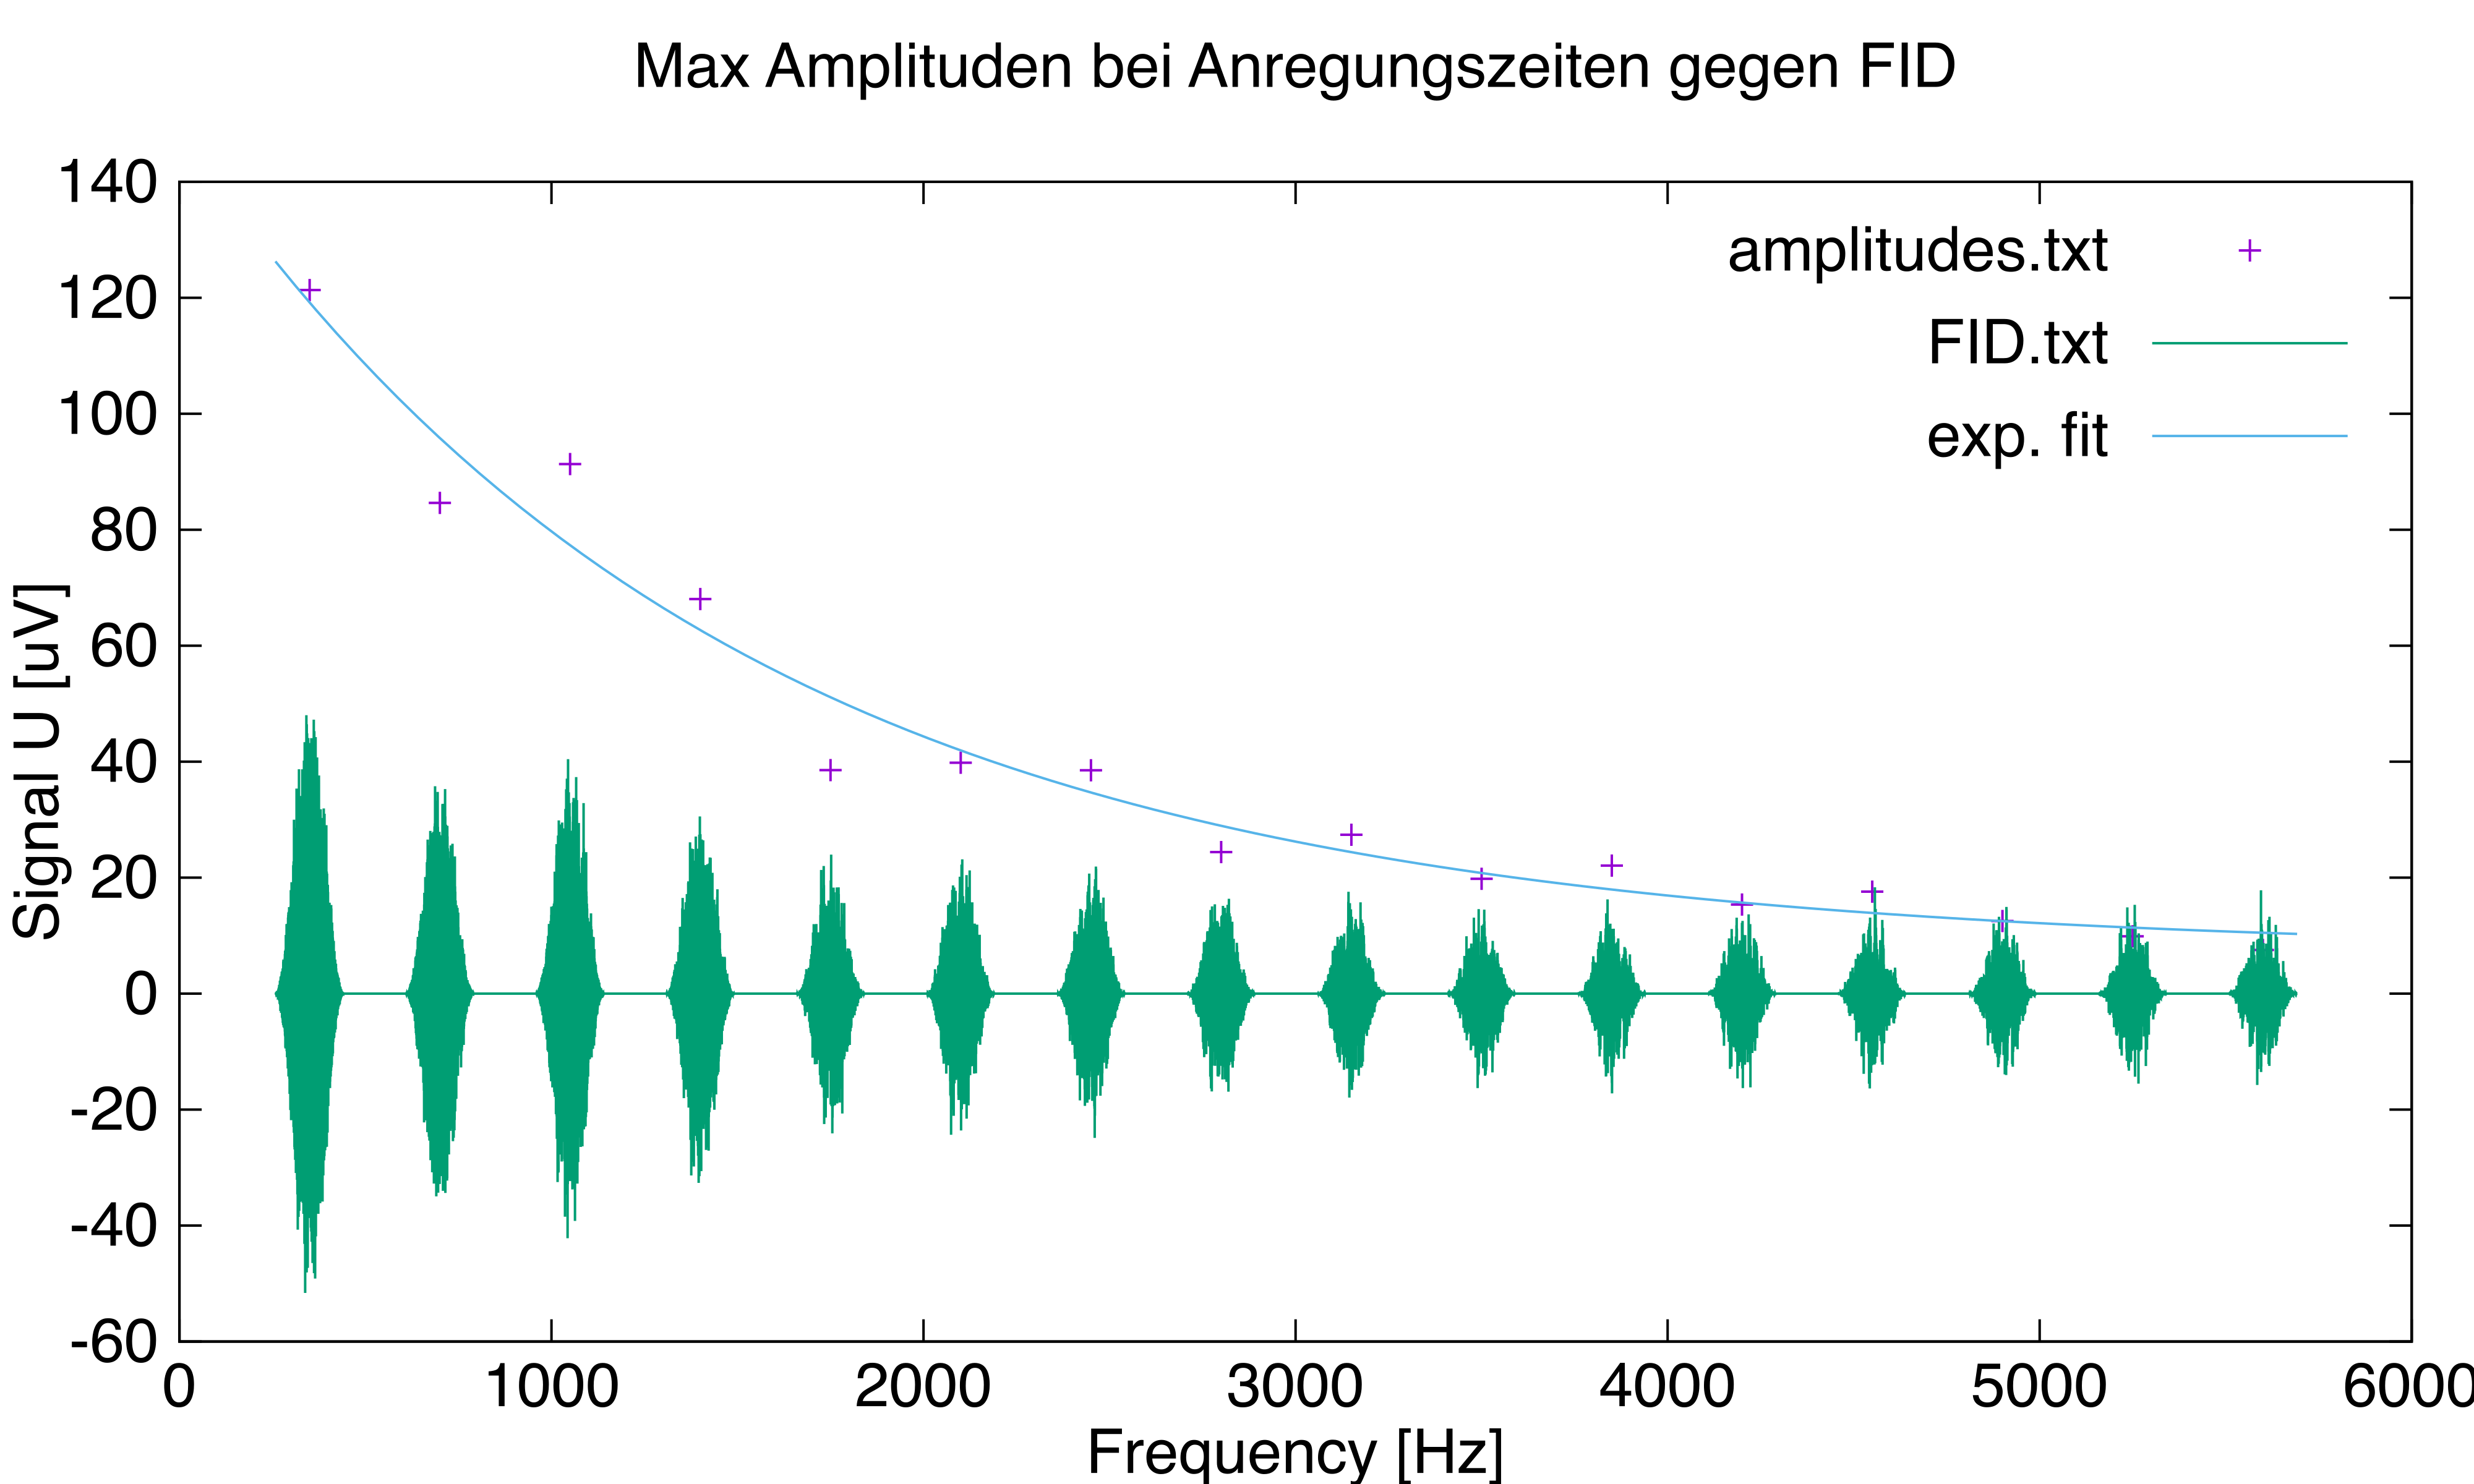
\includegraphics[width=6cm]{../Bilddateien/CPMG-0-0-constant-avg.png}
                \caption{mod. const.}
                \label{fig:CPMG-0-0-constant-avg}
            \end{subfigure}
            \
            \begin{subfigure}[b]{0.4\textwidth}
                \centering
                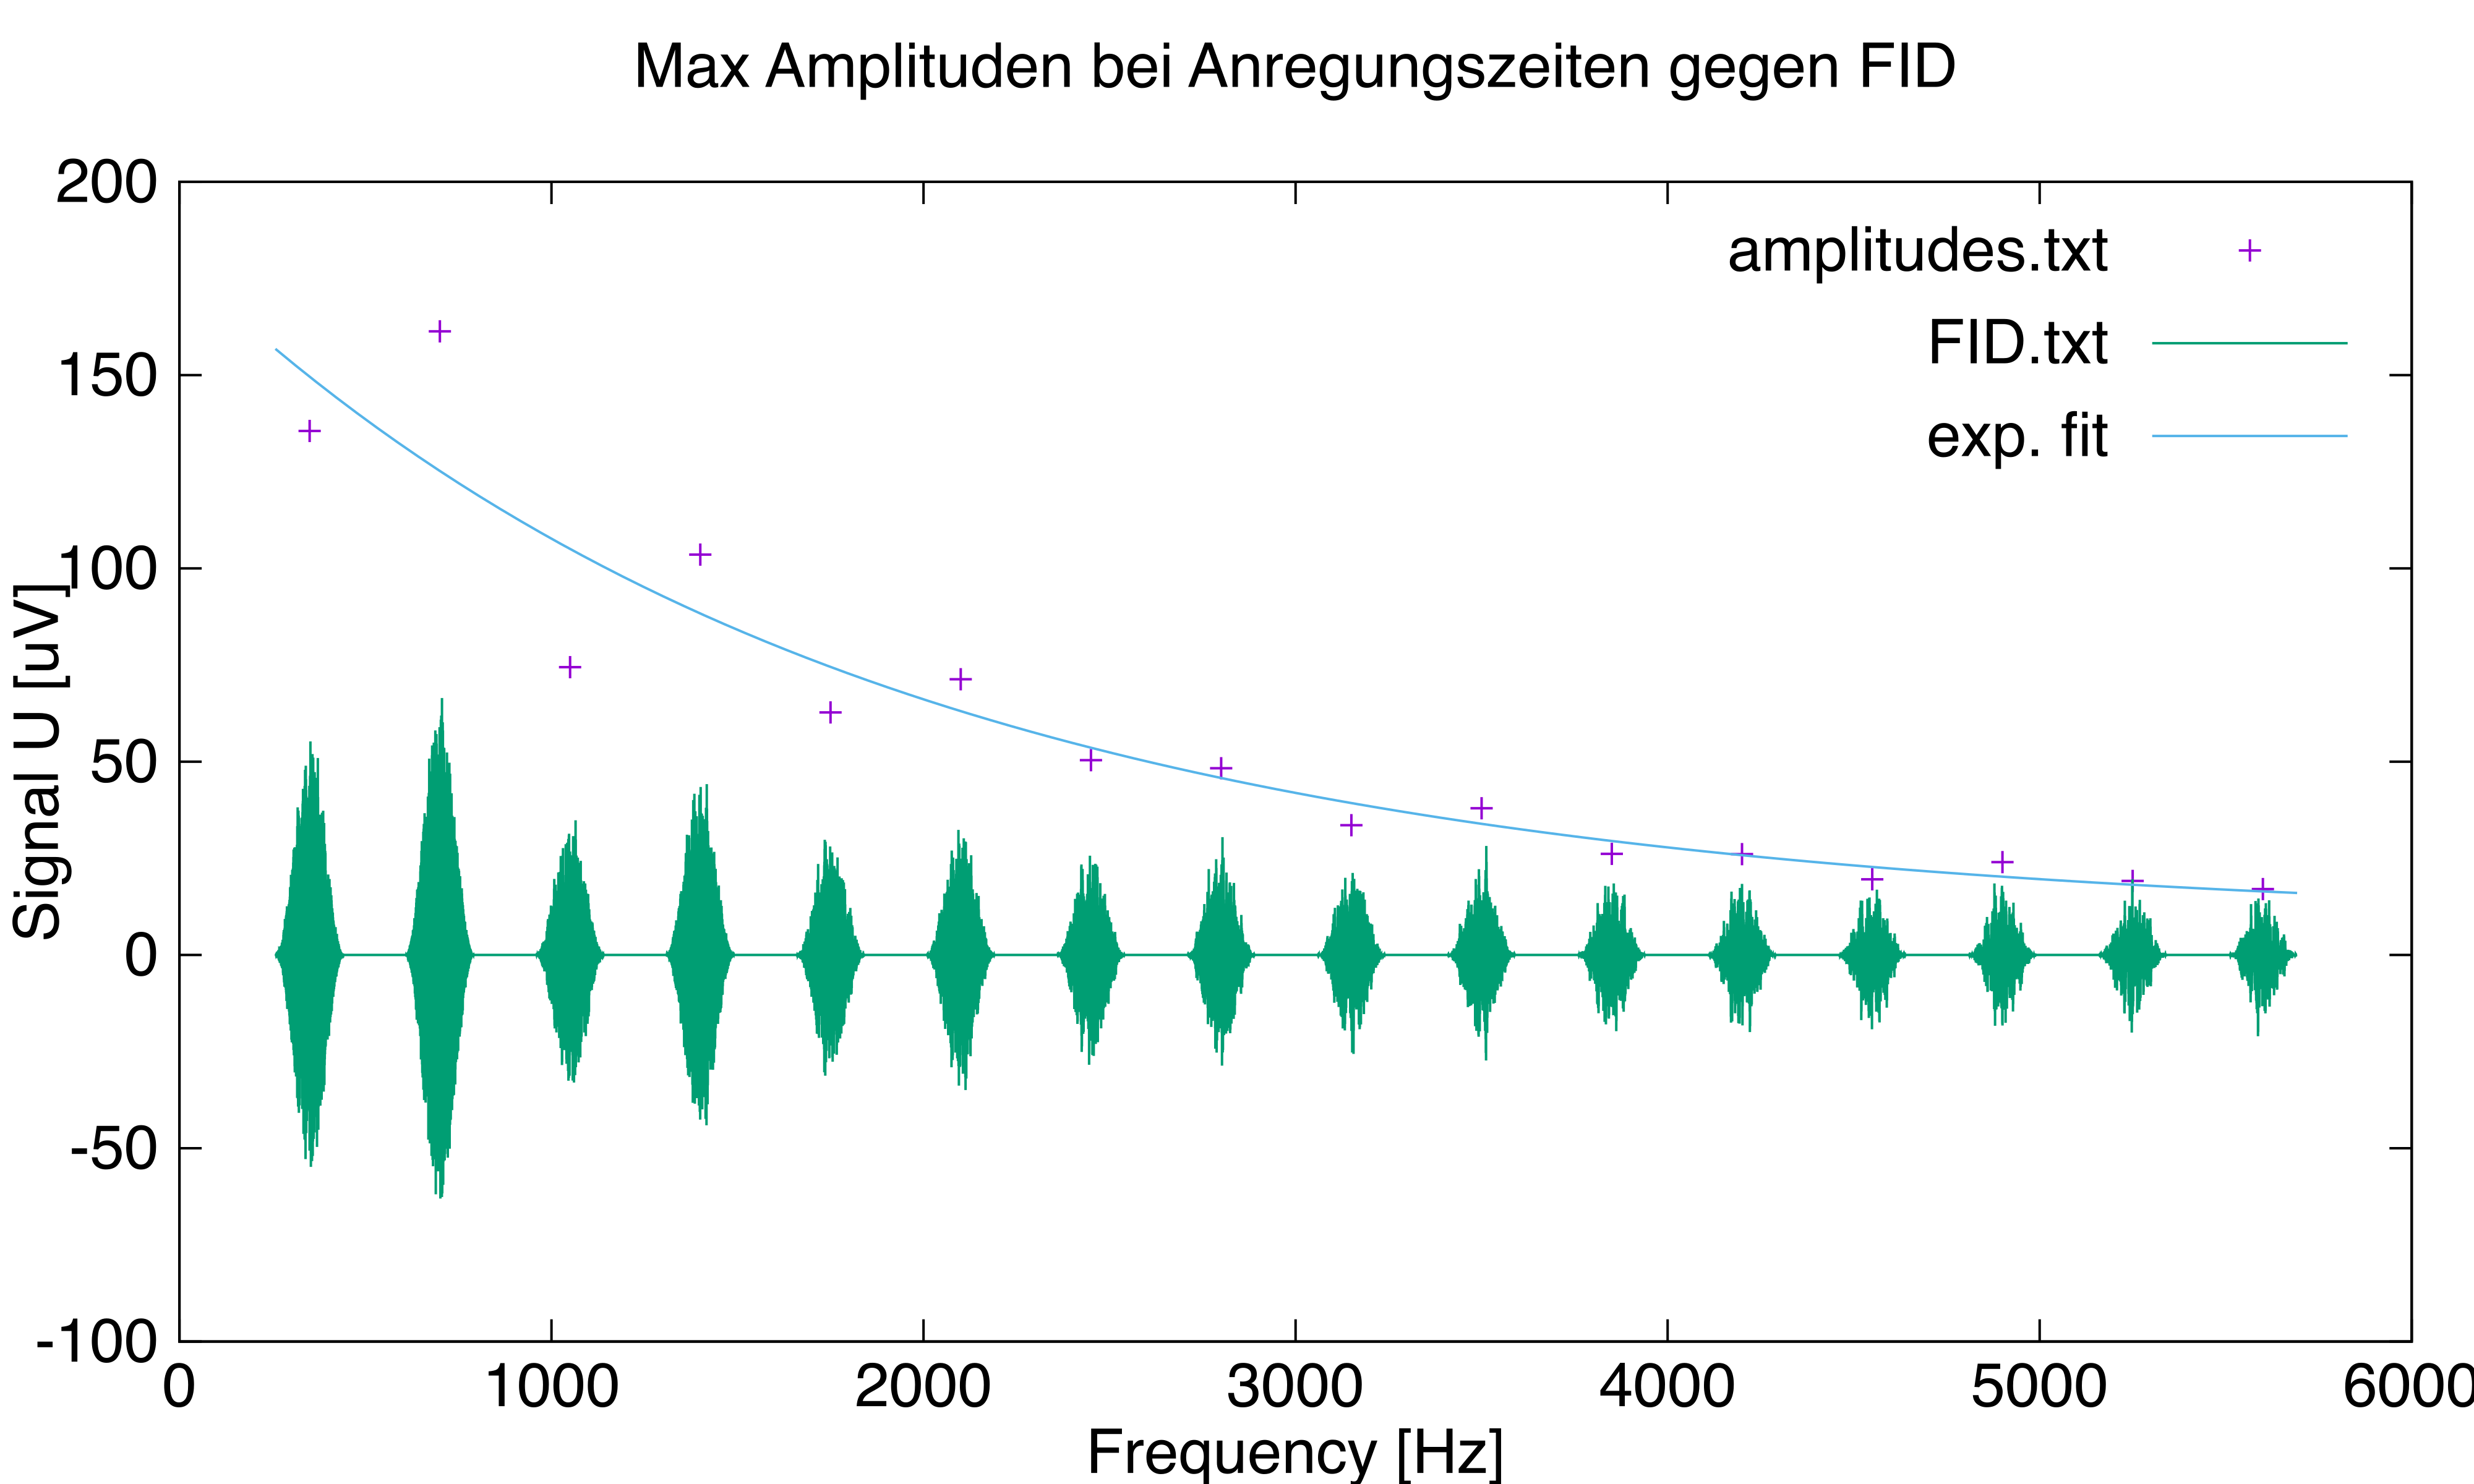
\includegraphics[width=6cm]{../Bilddateien/CPMG-0-0-alternating-avg.png}
                \caption{mod. alt.}
                \label{fig:CPMG-0-0-alternating-avg}
            \end{subfigure}
            \caption{FID und Amplitudensignale nichtnormiert und gemittelt für $\varphi_1 = 0$, $\varphi_2 = 0$.}
            \label{fig:CPMG-0-0-avg}
        \end{figure}

        \begin{figure}[h]
            \centering
            \begin{subfigure}[b]{0.4\textwidth}
                \centering
                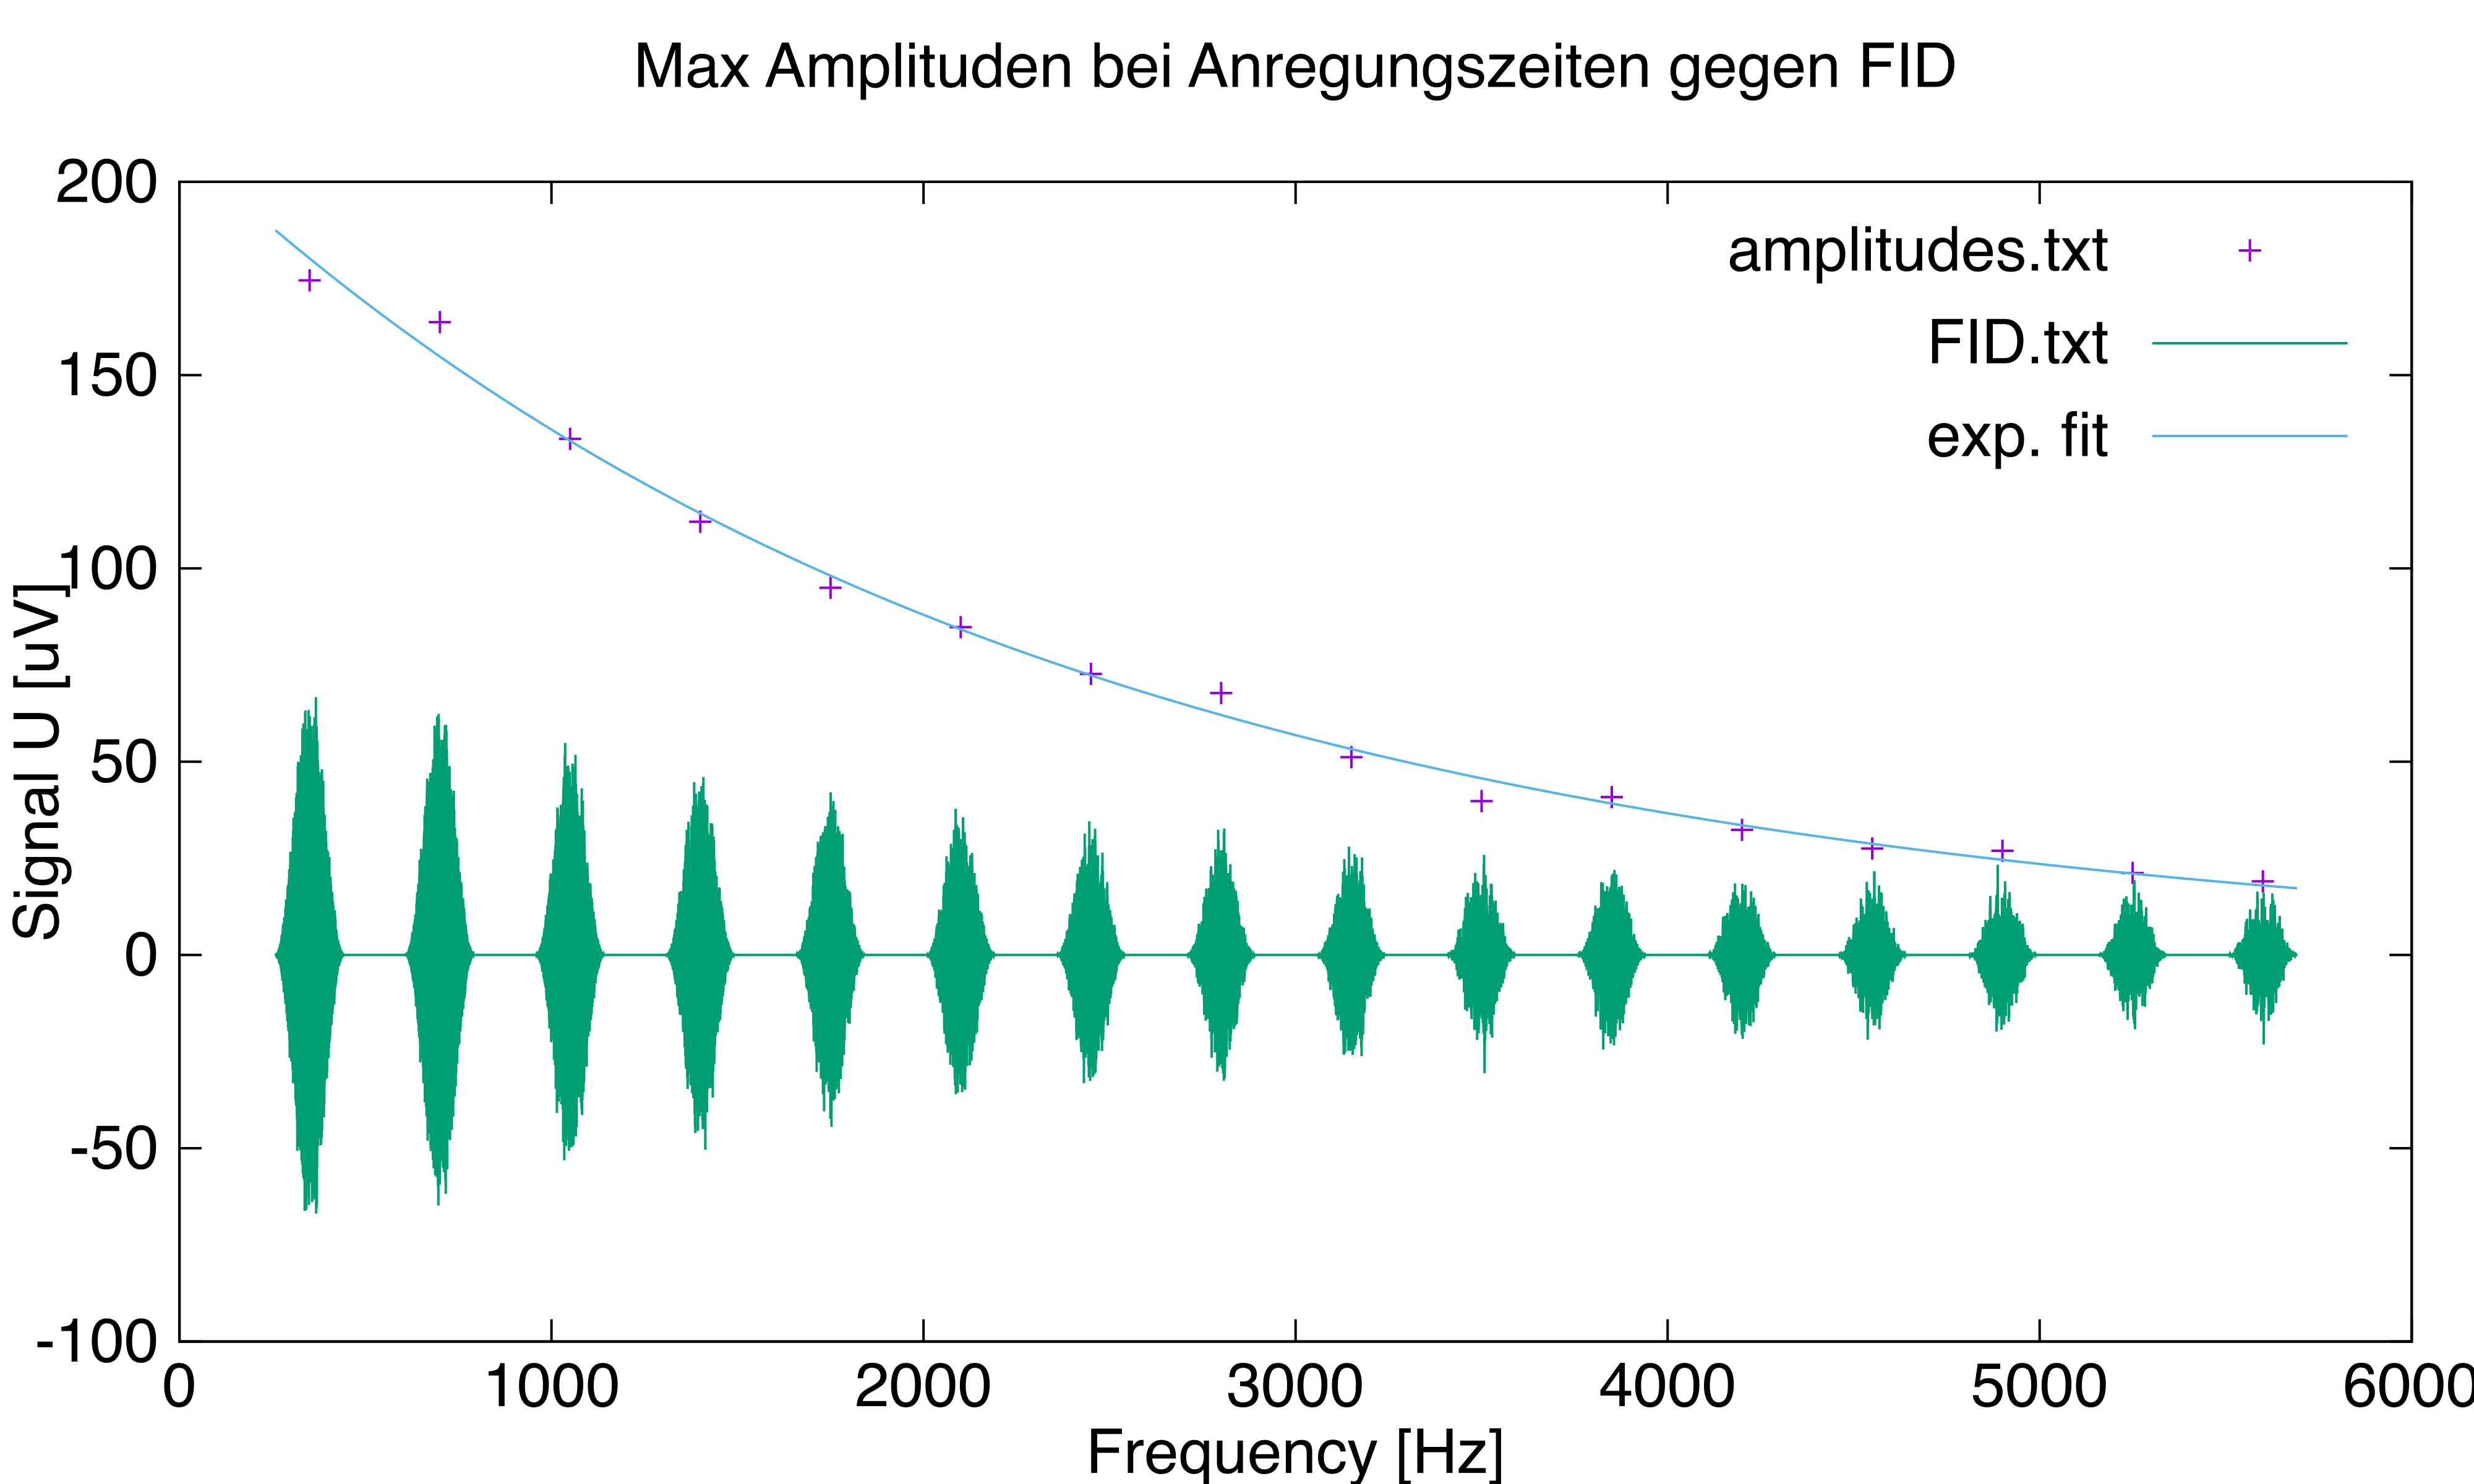
\includegraphics[width=6cm]{../Bilddateien/CPMG-0-90-constant-avg.png}
                \caption{mod. const.}
                \label{fig:CPMG-0-90-constant-avg}
            \end{subfigure}
            \
            \begin{subfigure}[b]{0.4\textwidth}
                \centering
                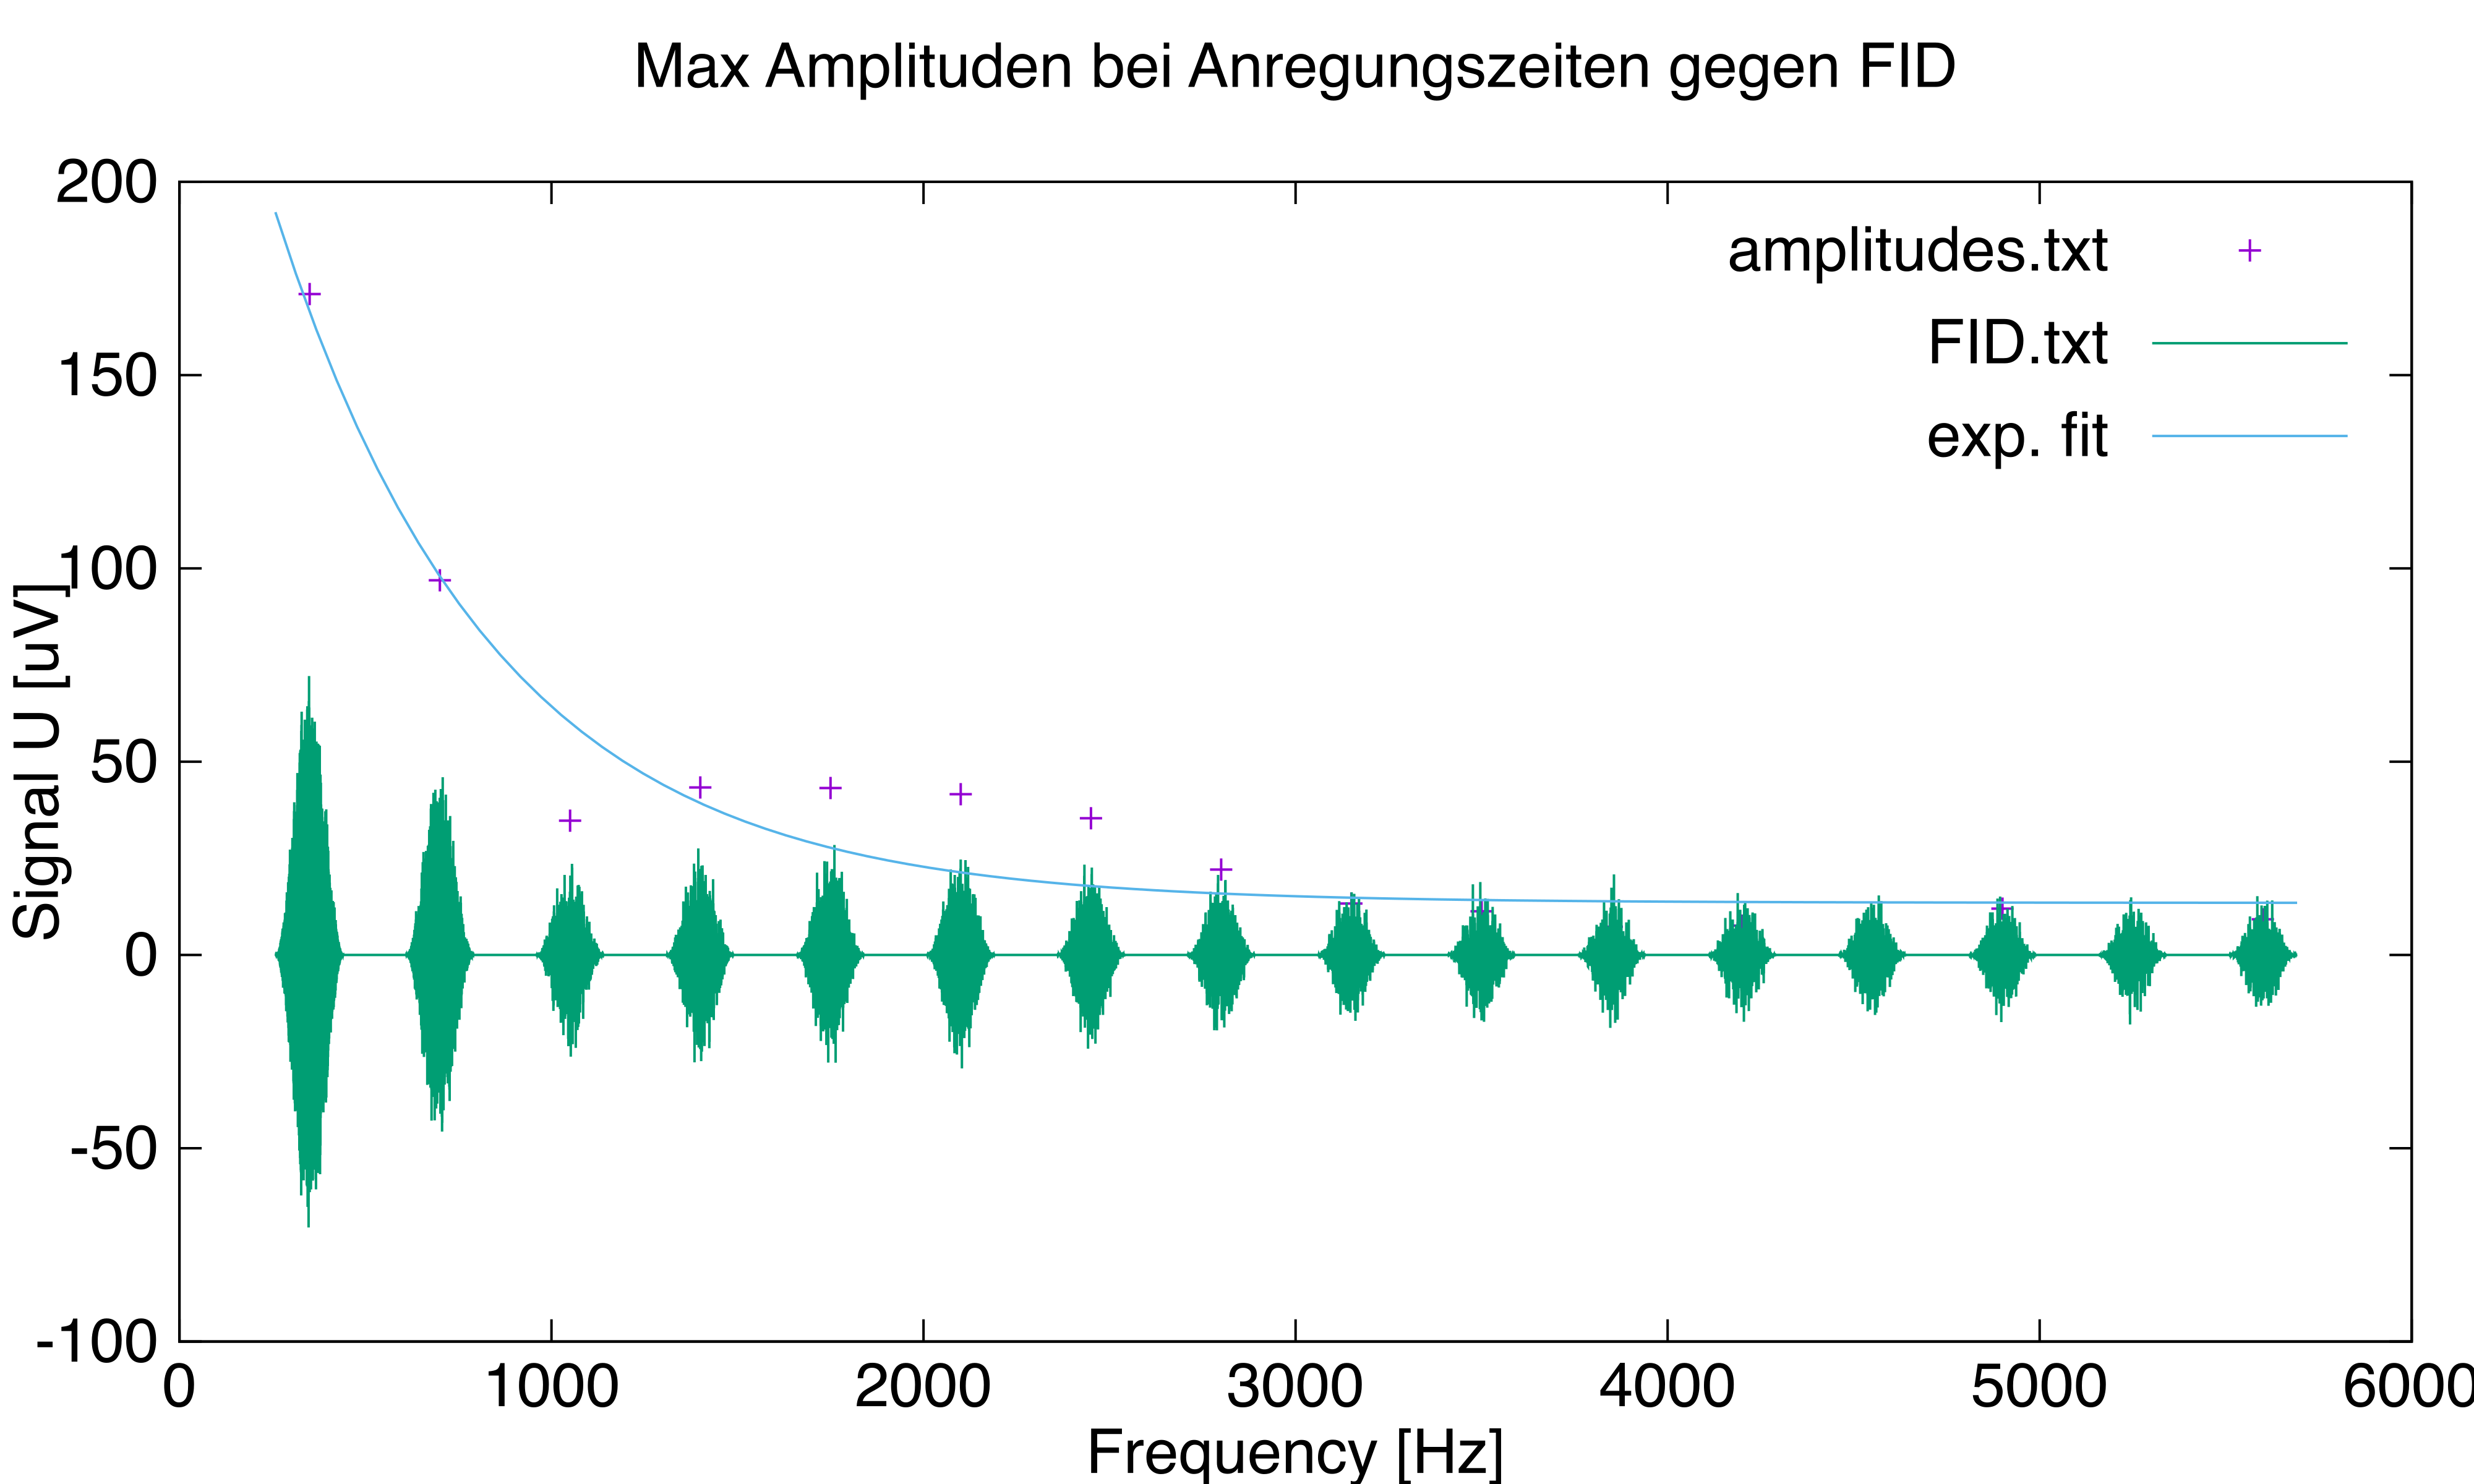
\includegraphics[width=6cm]{../Bilddateien/CPMG-0-90-alternating-avg.png}
                \caption{mod. alt.}
                \label{fig:CPMG-0-90-alternating-avg}
            \end{subfigure}
            \caption{FID und Amplitudensignale nichtnormiert und gemittelt für $\varphi_1 = 0$, $\varphi_2 = 90$.}
            \label{fig:CPMG-0-90-avg}
        \end{figure}
        
        \begin{figure}[h]
            \centering
            \begin{subfigure}[b]{0.4\textwidth}
                \centering
                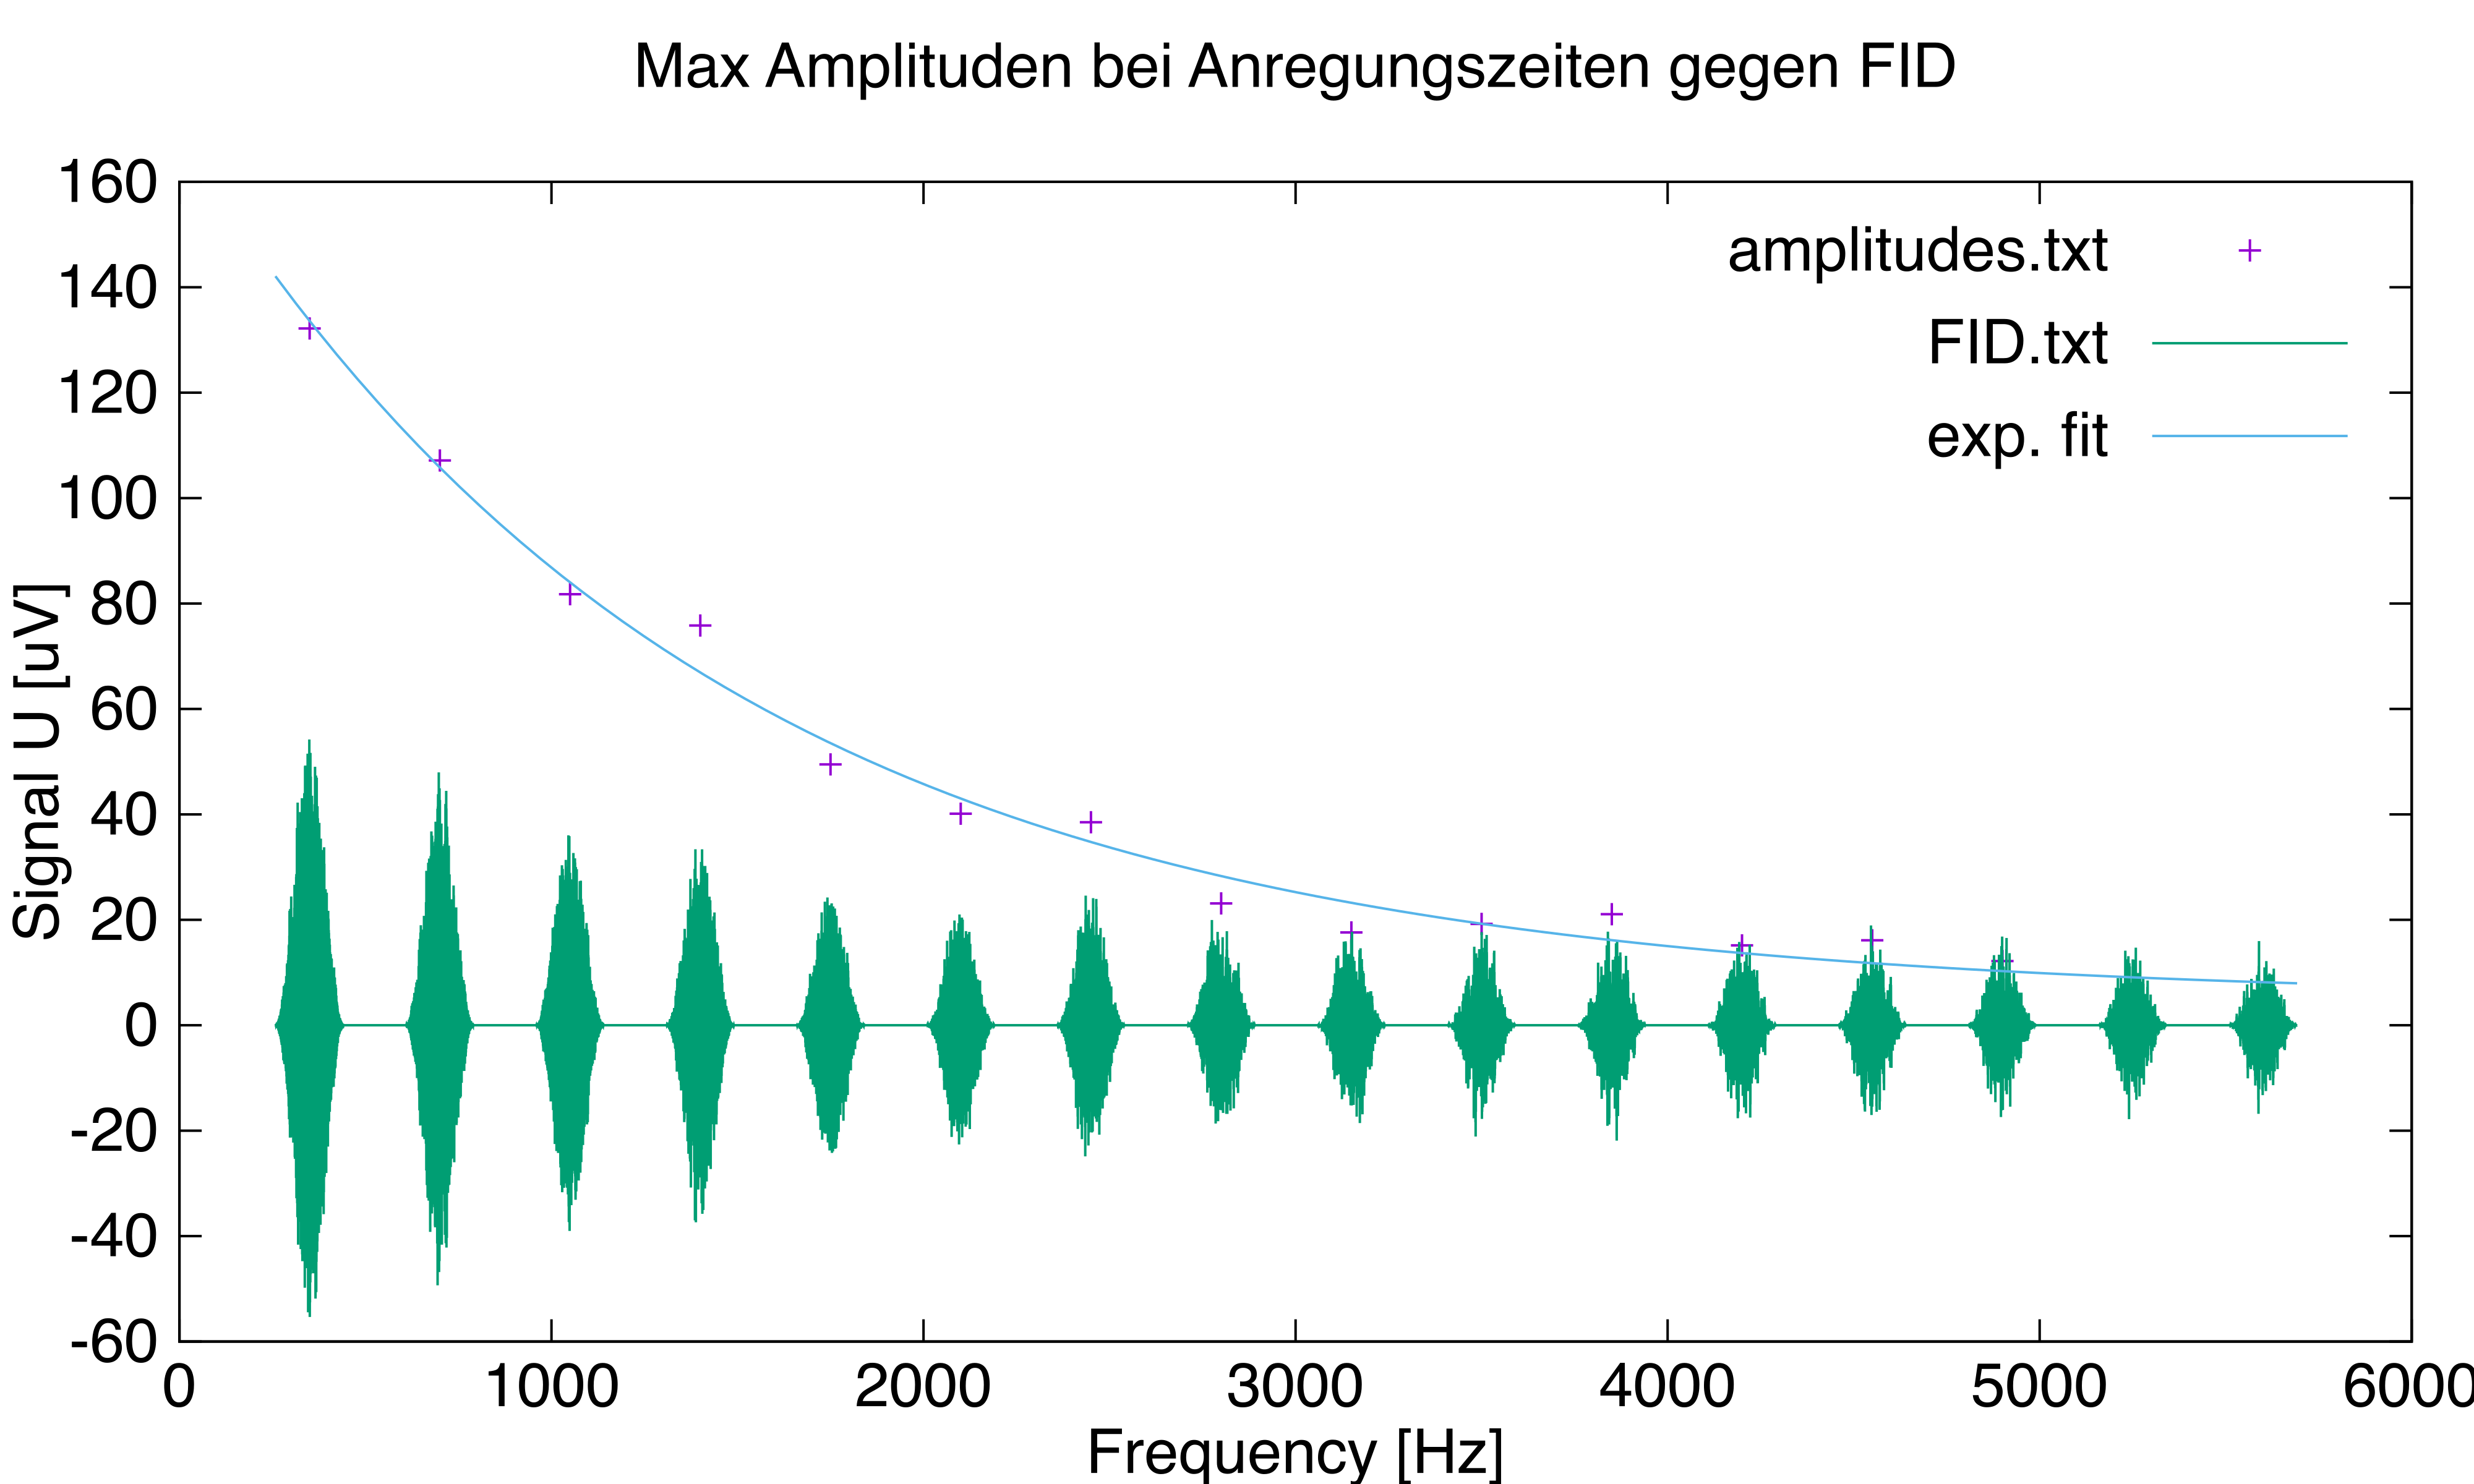
\includegraphics[width=6cm]{../Bilddateien/CPMG-0-180-constant-avg.png}
                \caption{mod. const.}
                \label{fig:CPMG-0-180-constant-avg}
            \end{subfigure}
            \
            \begin{subfigure}[b]{0.4\textwidth}
                \centering
                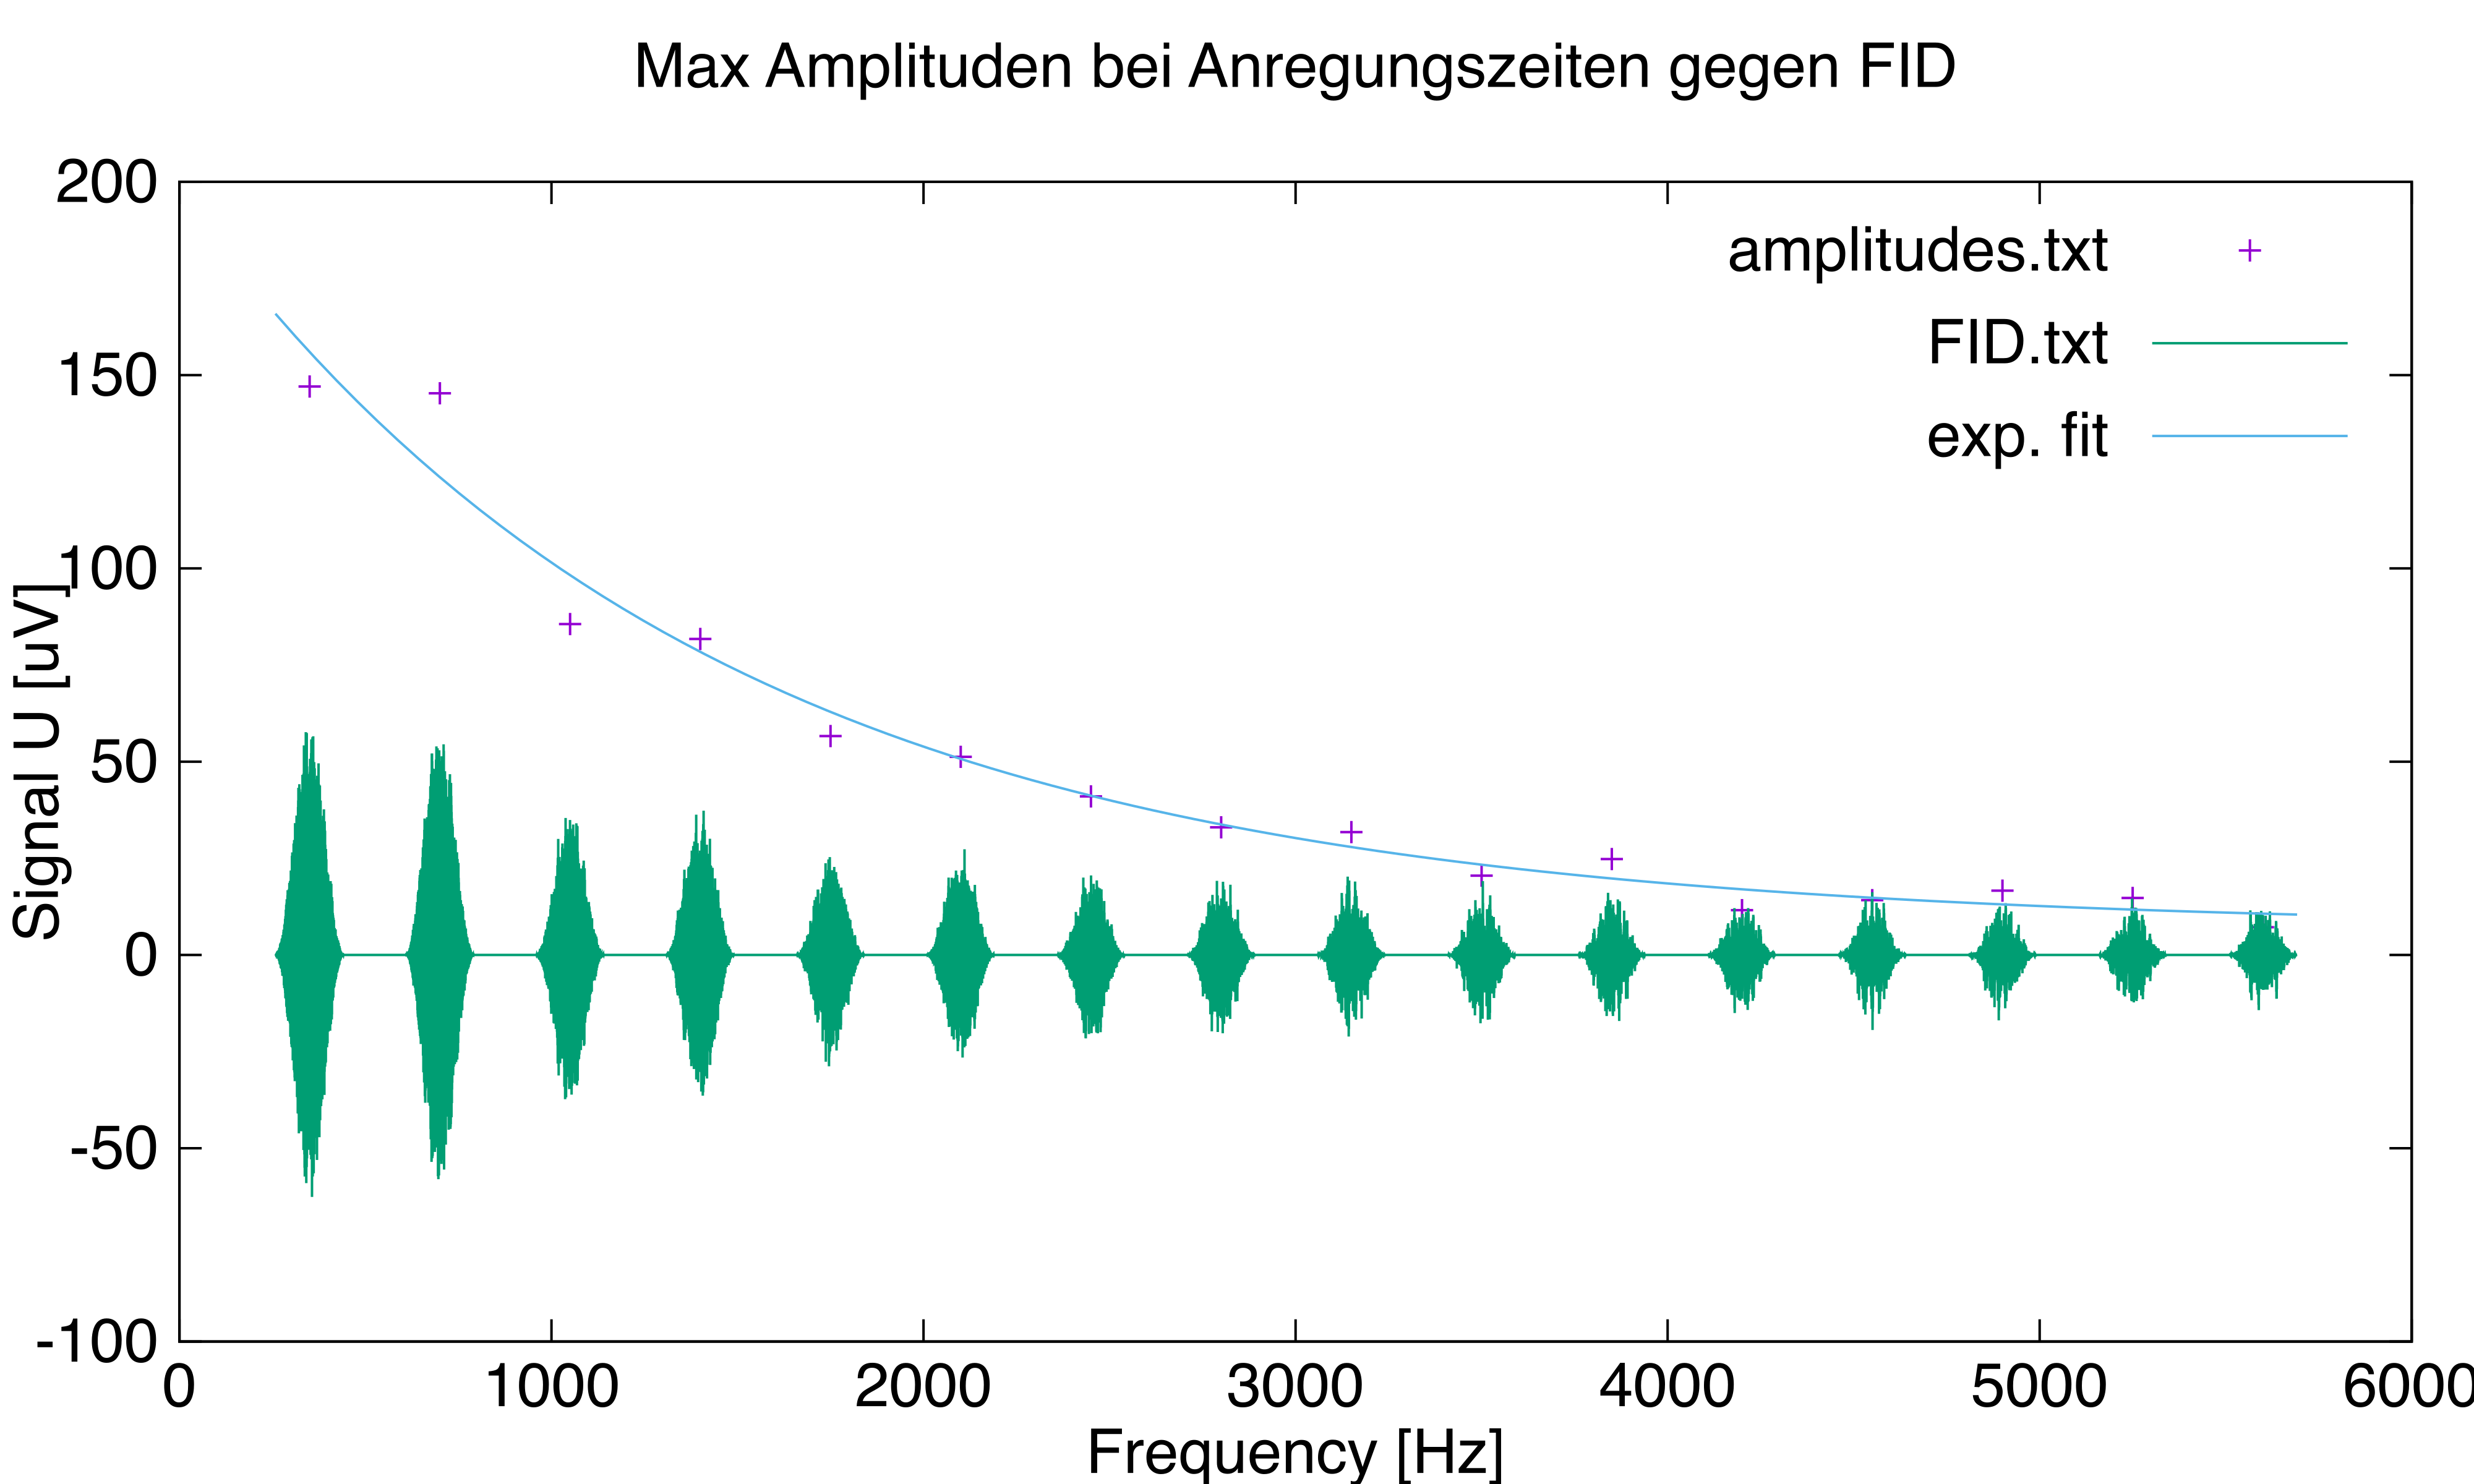
\includegraphics[width=6cm]{../Bilddateien/CPMG-0-180-alternating-avg.png}
                \caption{mod. alt.}
                \label{fig:CPMG-0-180-alternating-avg}
            \end{subfigure}
            \caption{FID und Amplitudensignale nichtnormiert und gemittelt für $\varphi_1 = 0$, $\varphi_2 = 180$.}
            \label{fig:CPMG-0-180-avg}
        \end{figure}

        \begin{figure}[h]
            \centering
            \begin{subfigure}[b]{0.4\textwidth}
                \centering
                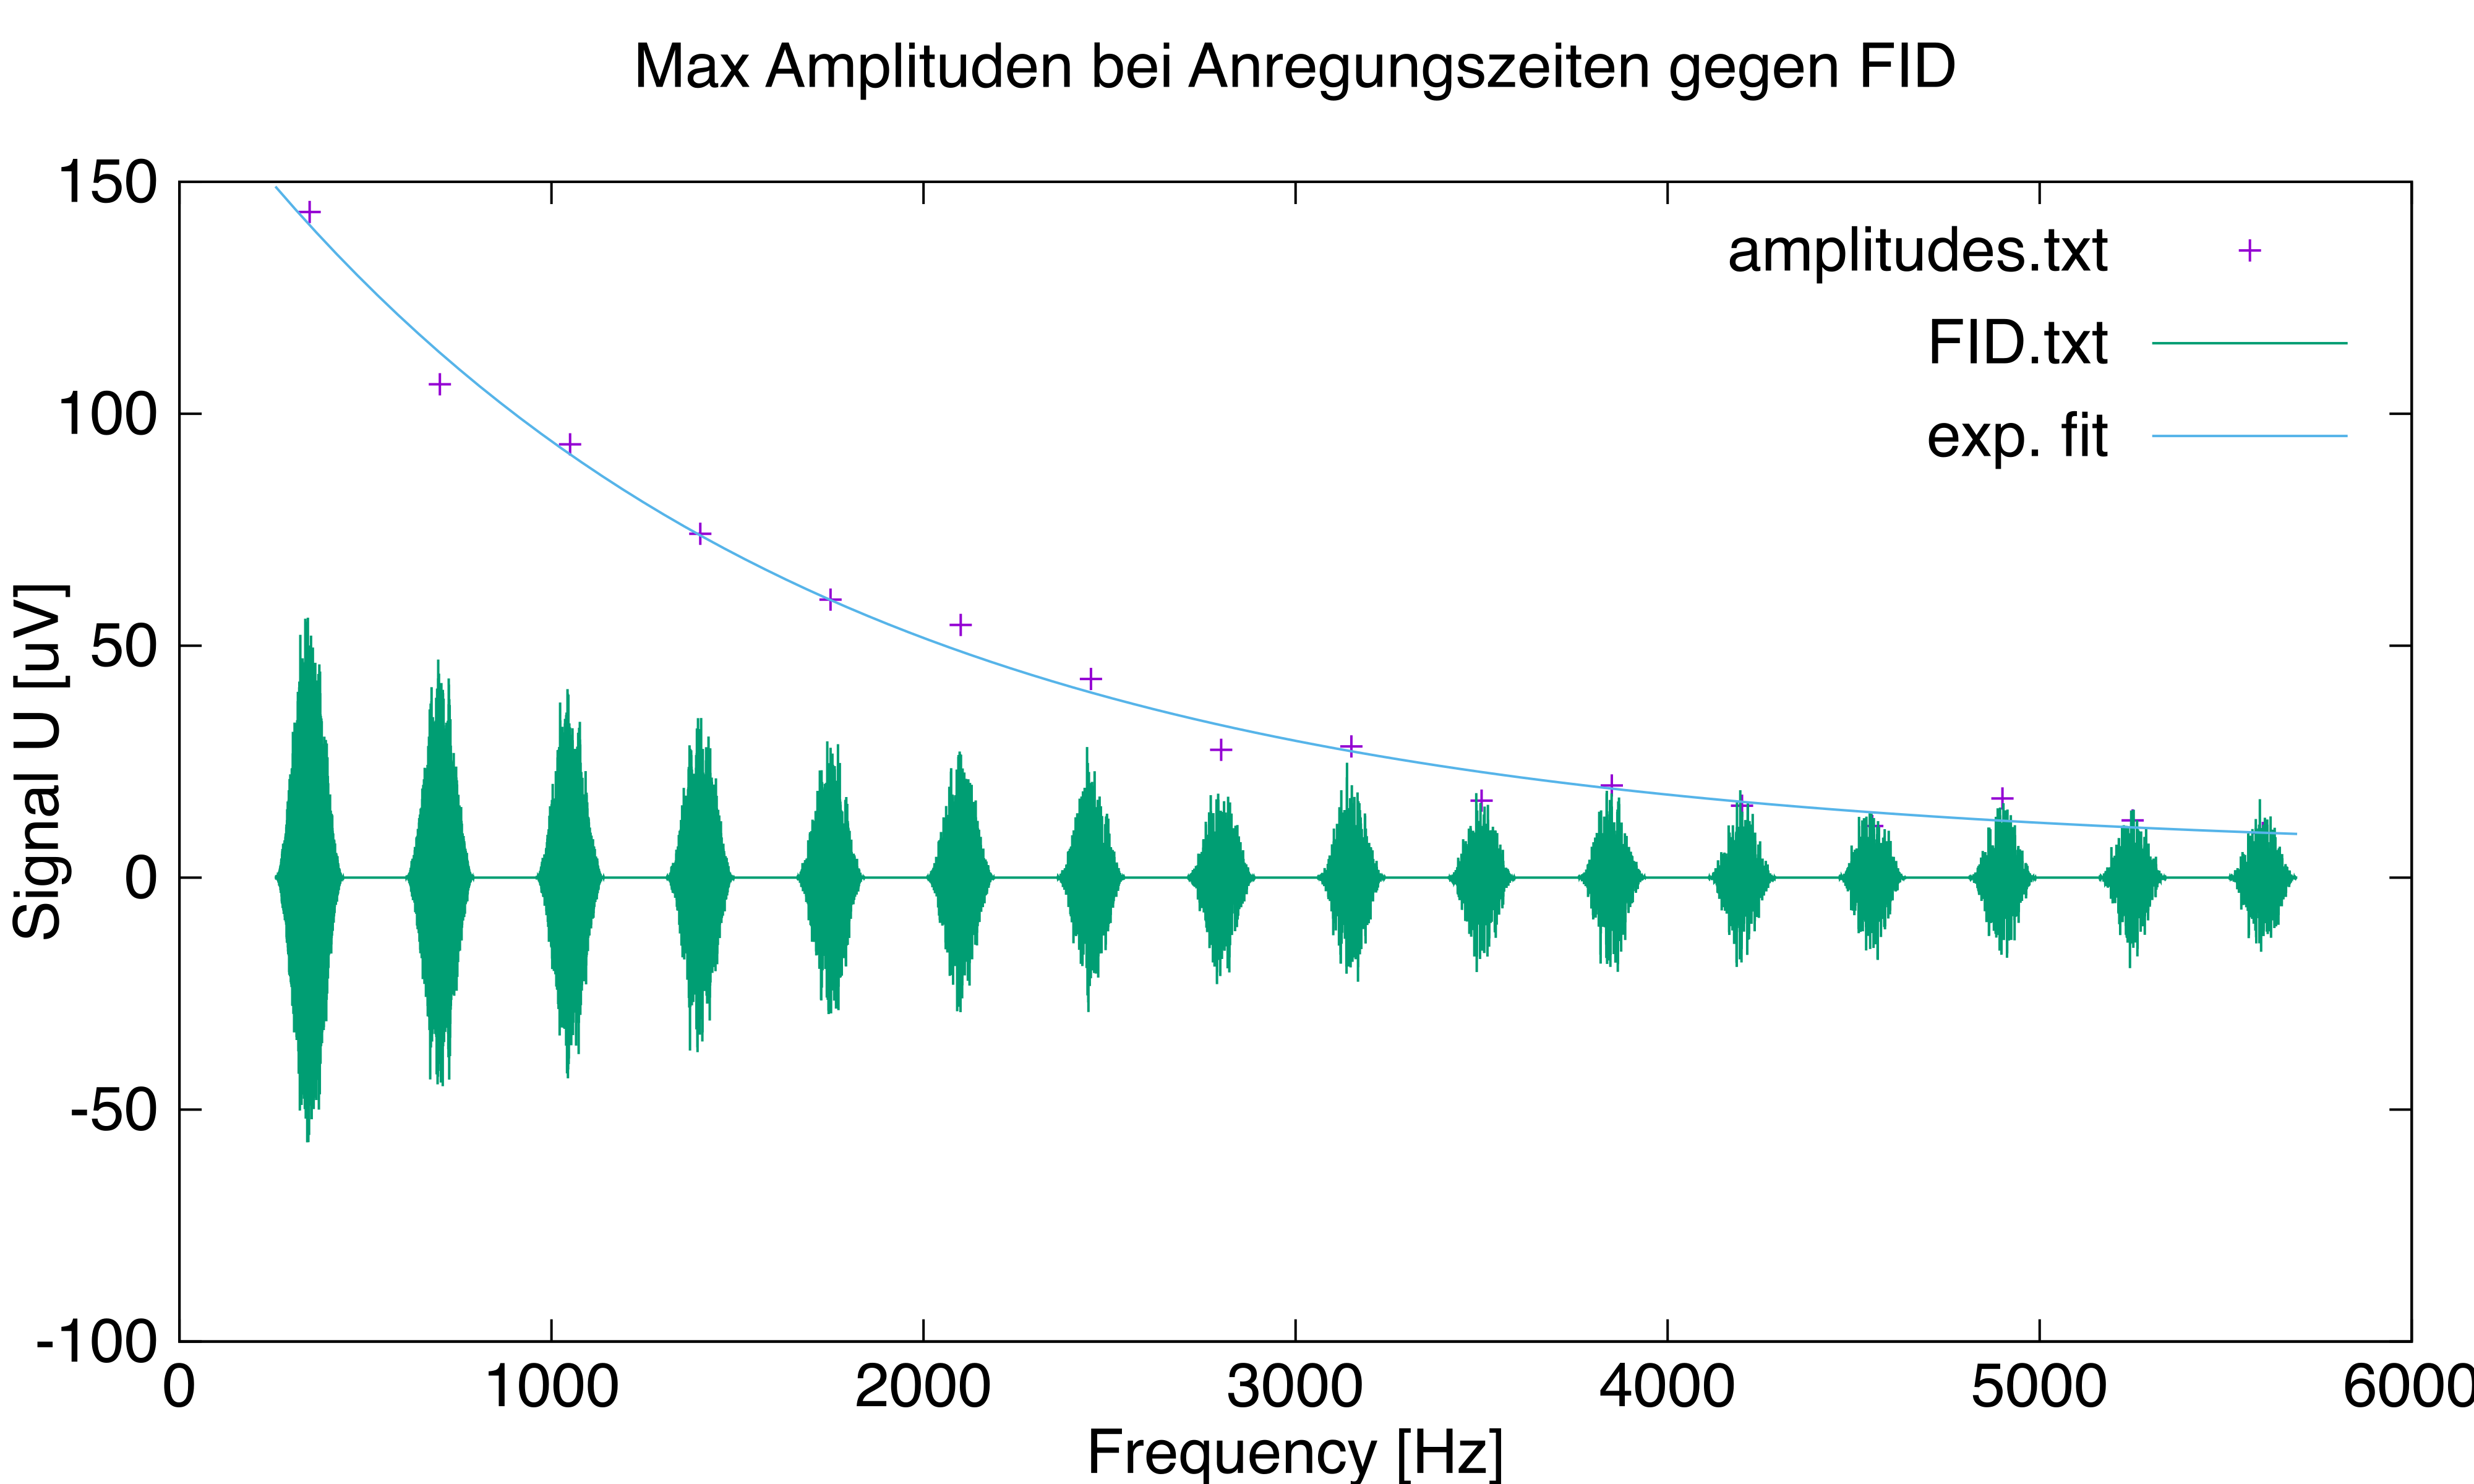
\includegraphics[width=6cm]{../Bilddateien/CPMG-90-0-constant-avg.png}
                \caption{mod. const.}
                \label{fig:CPMG-90-0-constant-avg}
            \end{subfigure}
            \
            \begin{subfigure}[b]{0.4\textwidth}
                \centering
                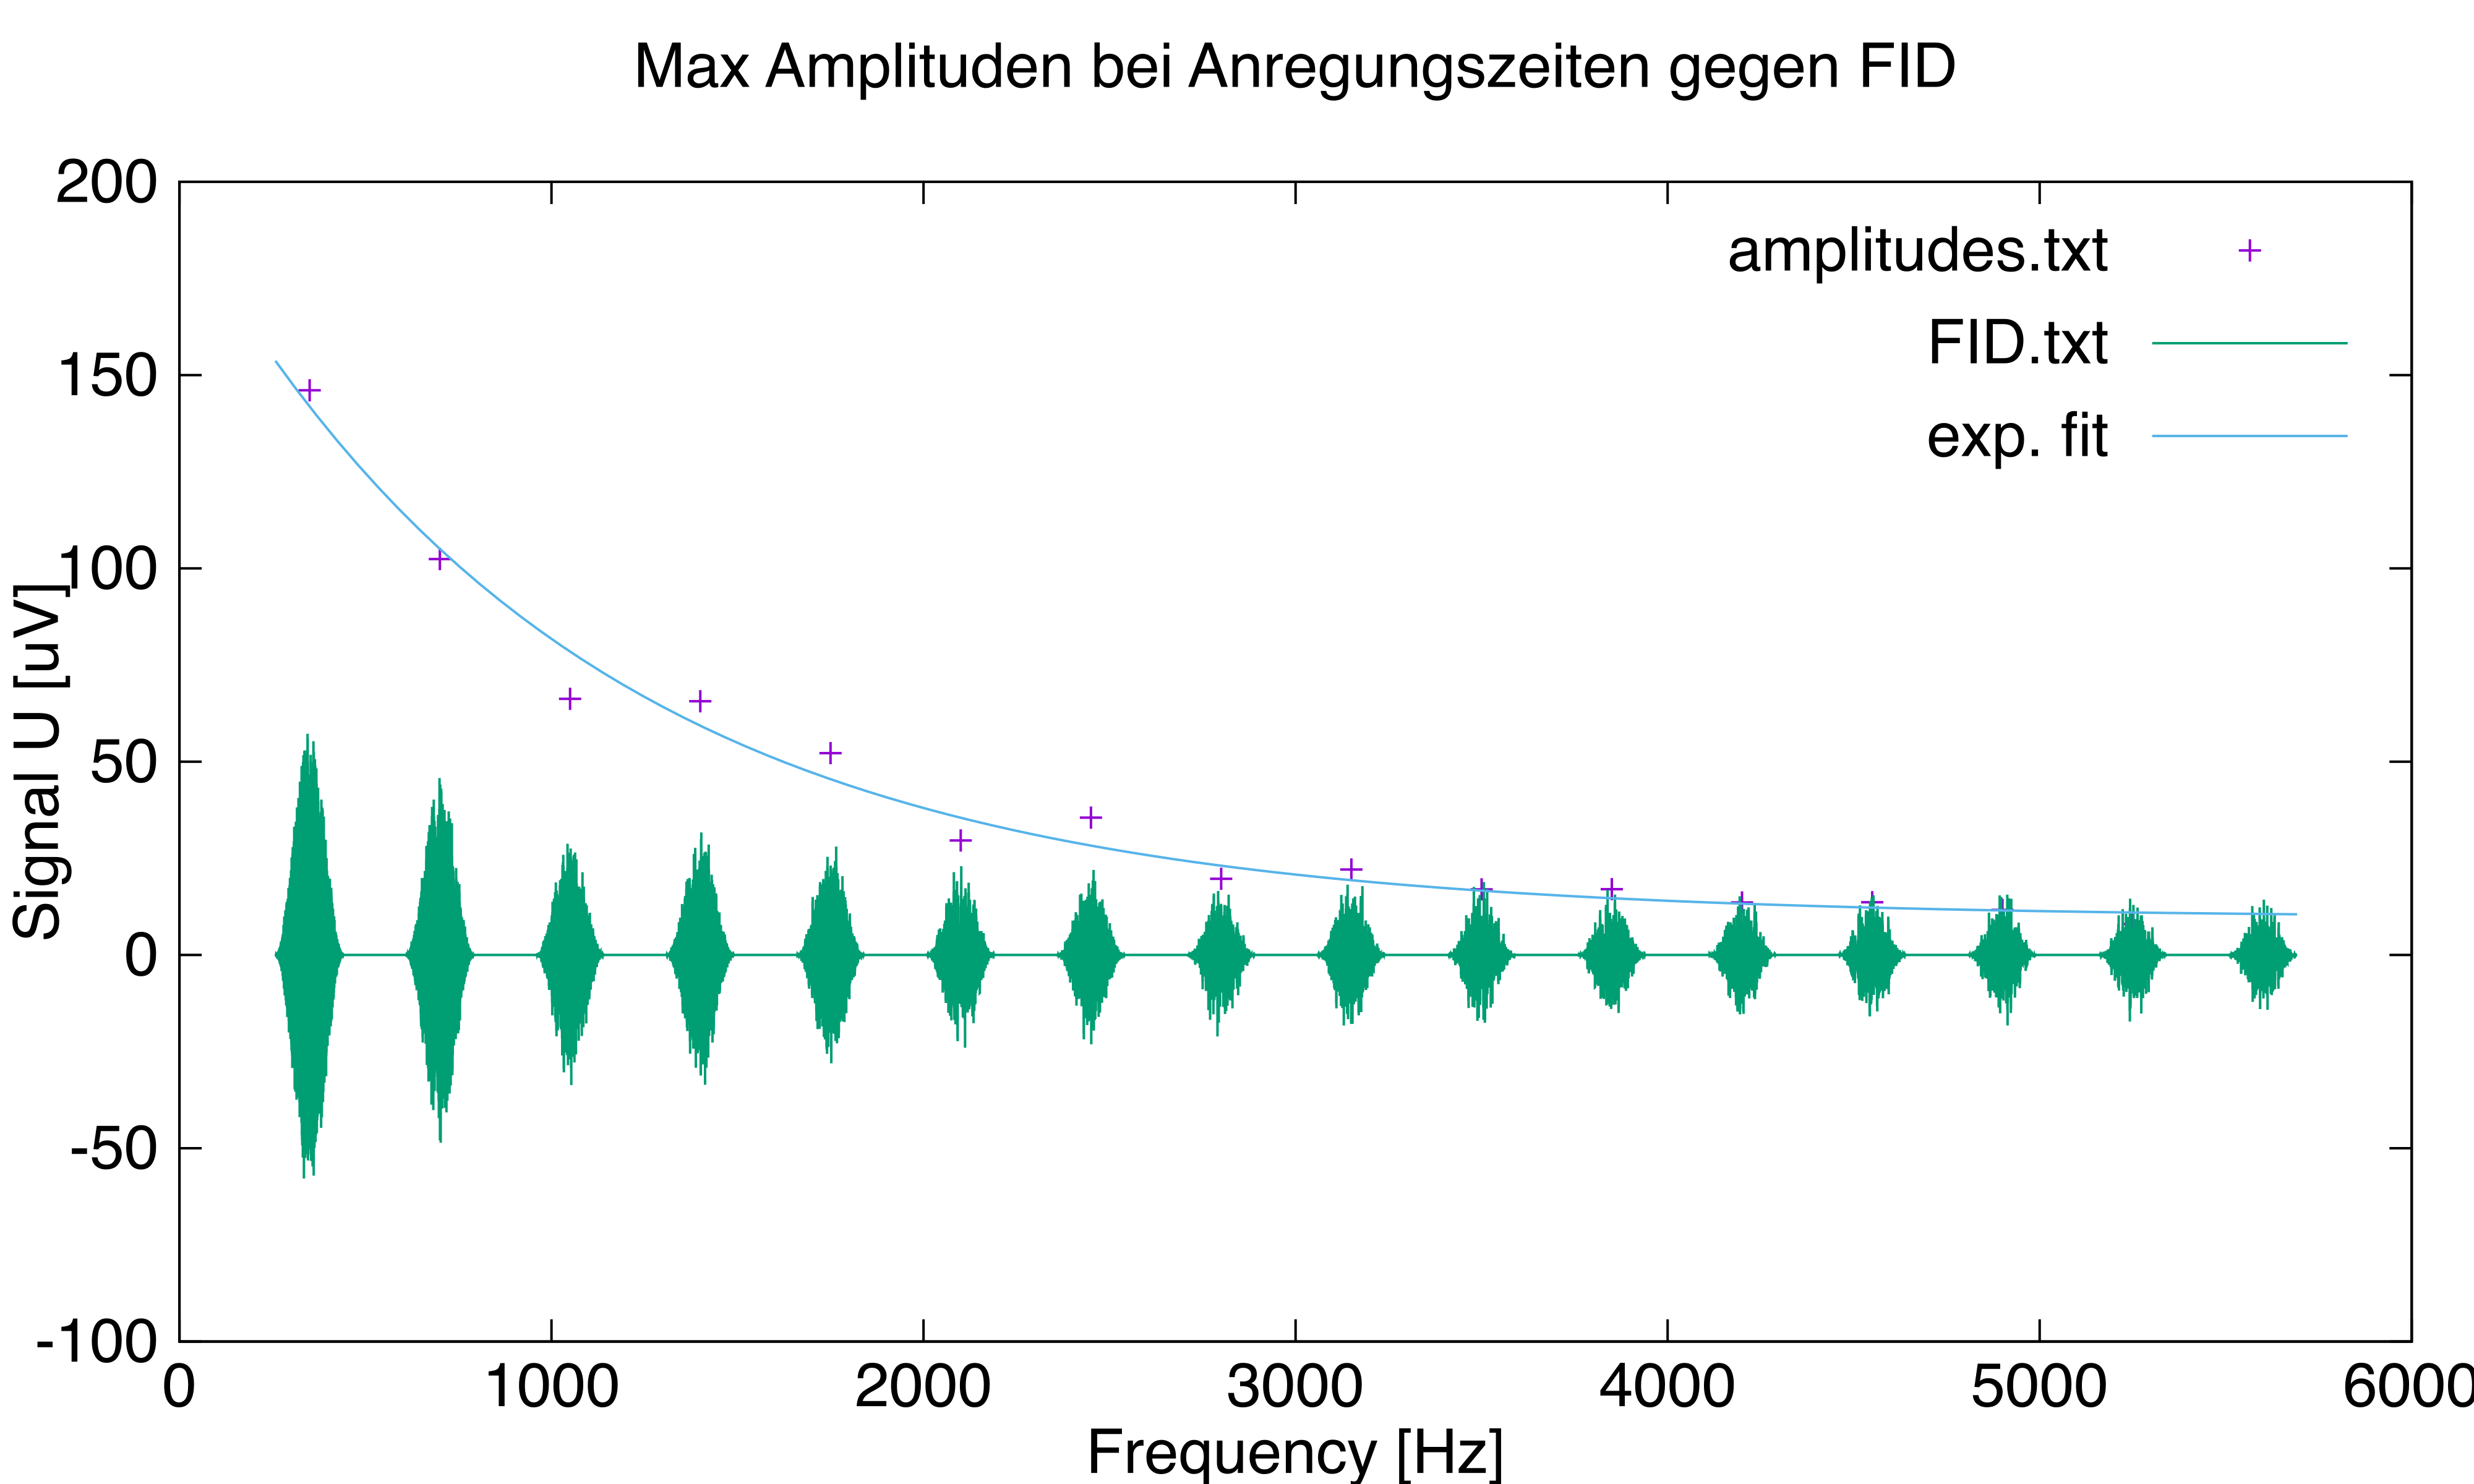
\includegraphics[width=6cm]{../Bilddateien/CPMG-90-0-alternating-avg.png}
                \caption{mod. alt.}
                \label{fig:CPMG-90-0-alternating-avg}
            \end{subfigure}
            \caption{FID und Amplitudensignale nichtnormiert und gemittelt für $\varphi_1 = 90$, $\varphi_2 = 0$.}
            \label{fig:CPMG-90-0-avg}
        \end{figure}

        \begin{figure}[h]
            \centering
            \begin{subfigure}[b]{0.4\textwidth}
                \centering
                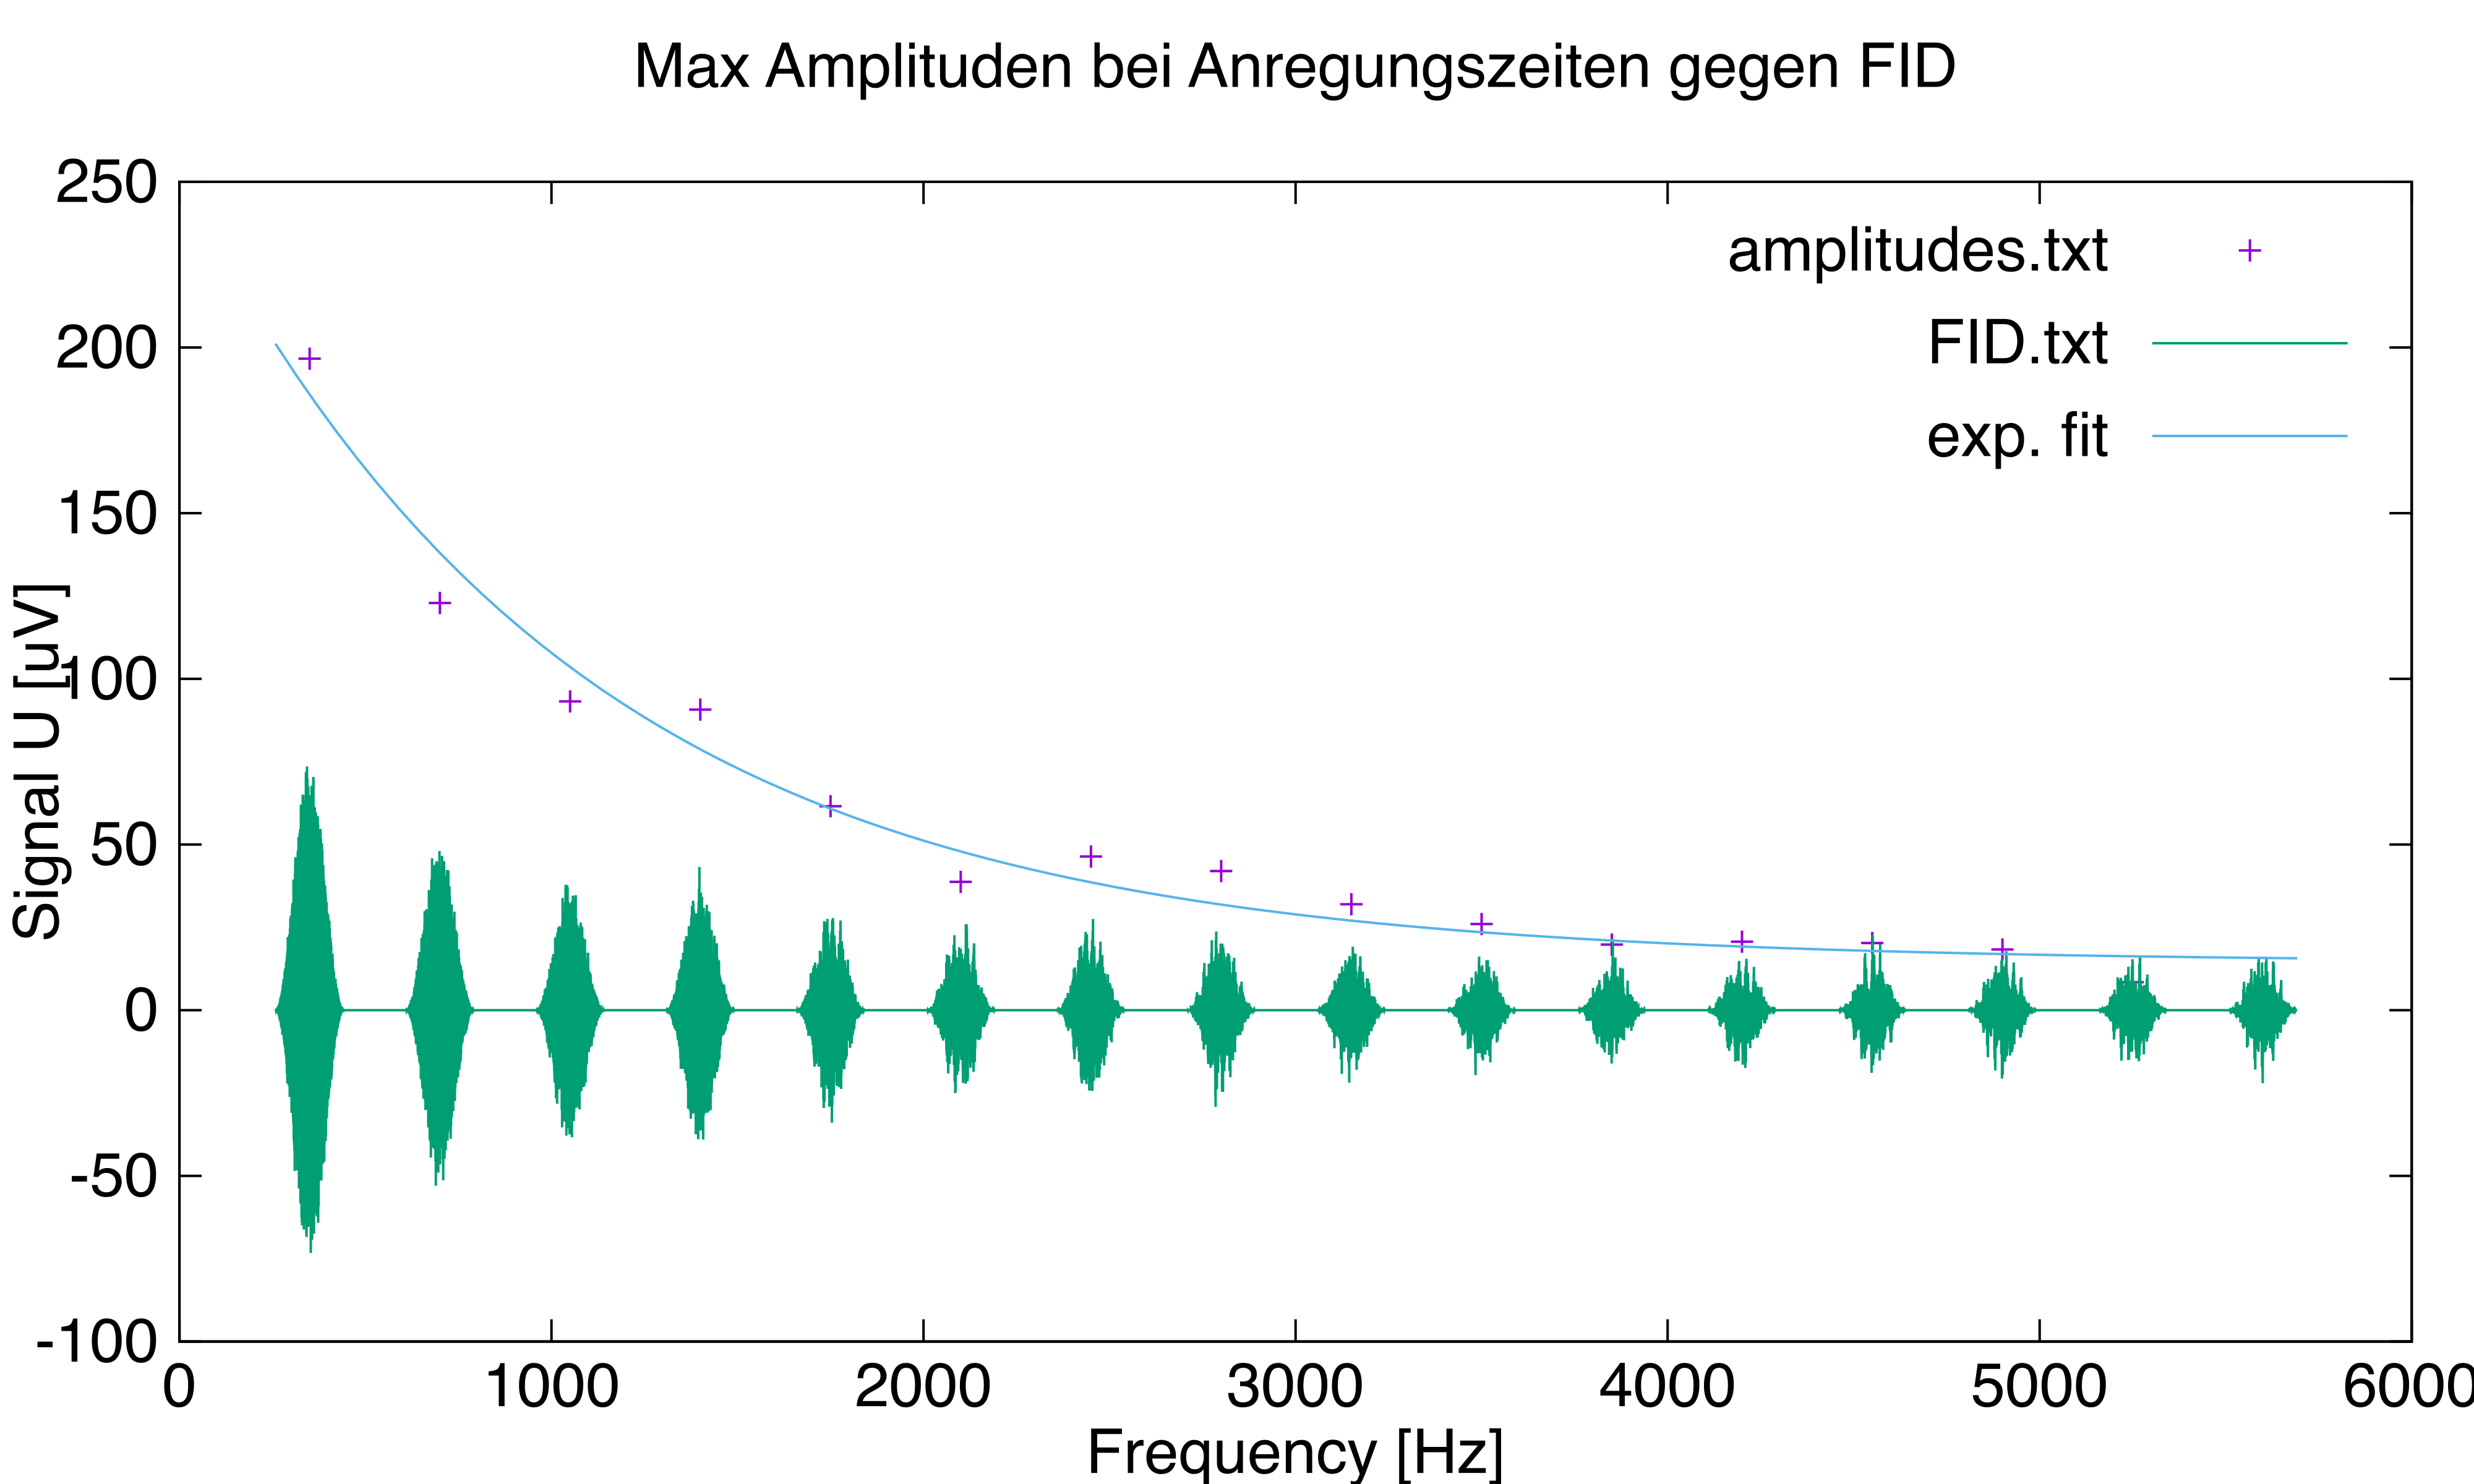
\includegraphics[width=6cm]{../Bilddateien/CPMG-180-0-constant-avg.png}
                \caption{mod. const.}
                \label{fig:CPMG-180-0-constant-avg}
            \end{subfigure}
            \
            \begin{subfigure}[b]{0.4\textwidth}
                \centering
                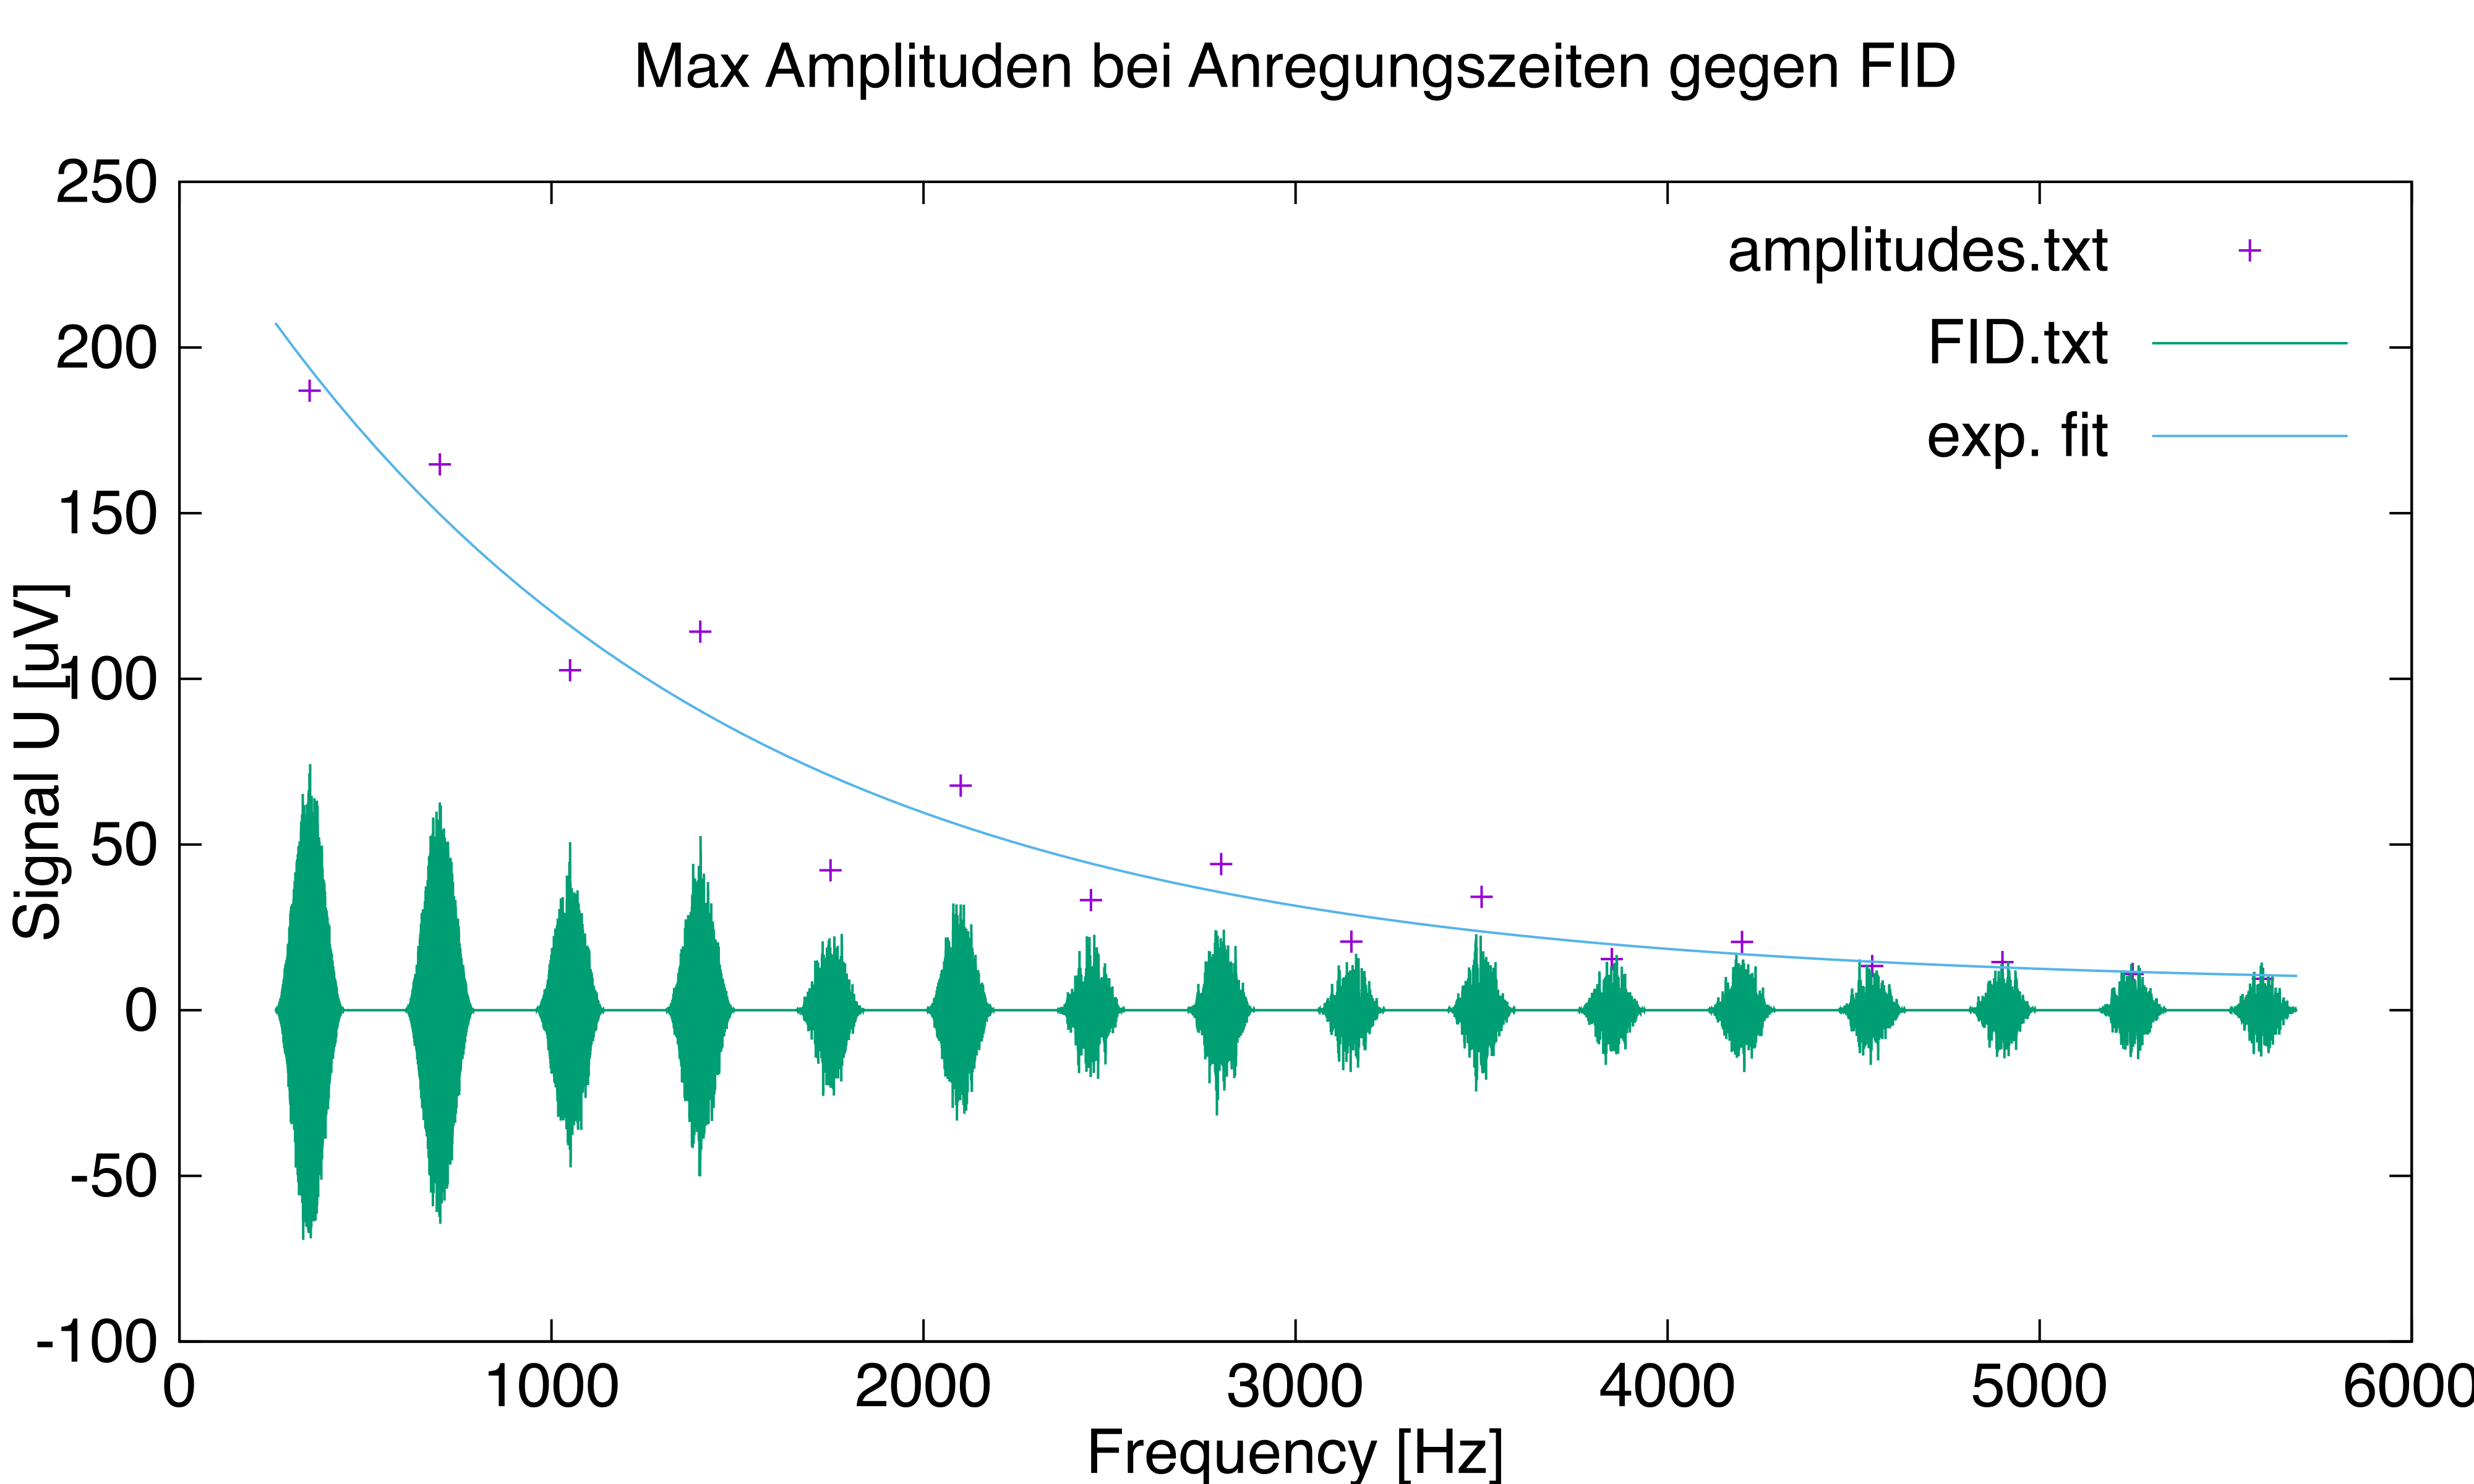
\includegraphics[width=6cm]{../Bilddateien/CPMG-180-0-alternating-avg.png}
                \caption{mod. alt.}
                \label{fig:CPMG-180-0-alternating-avg}
            \end{subfigure}
            \caption{FID und Amplitudensignale nichtnormiert und gemittelt für $\varphi_1 = 180$, $\varphi_2 = 0$.}
            \label{fig:CPMG-180-0-avg}
        \end{figure}

        \begin{figure}[h]
            \centering
            \begin{subfigure}[b]{0.4\textwidth}
                \centering
                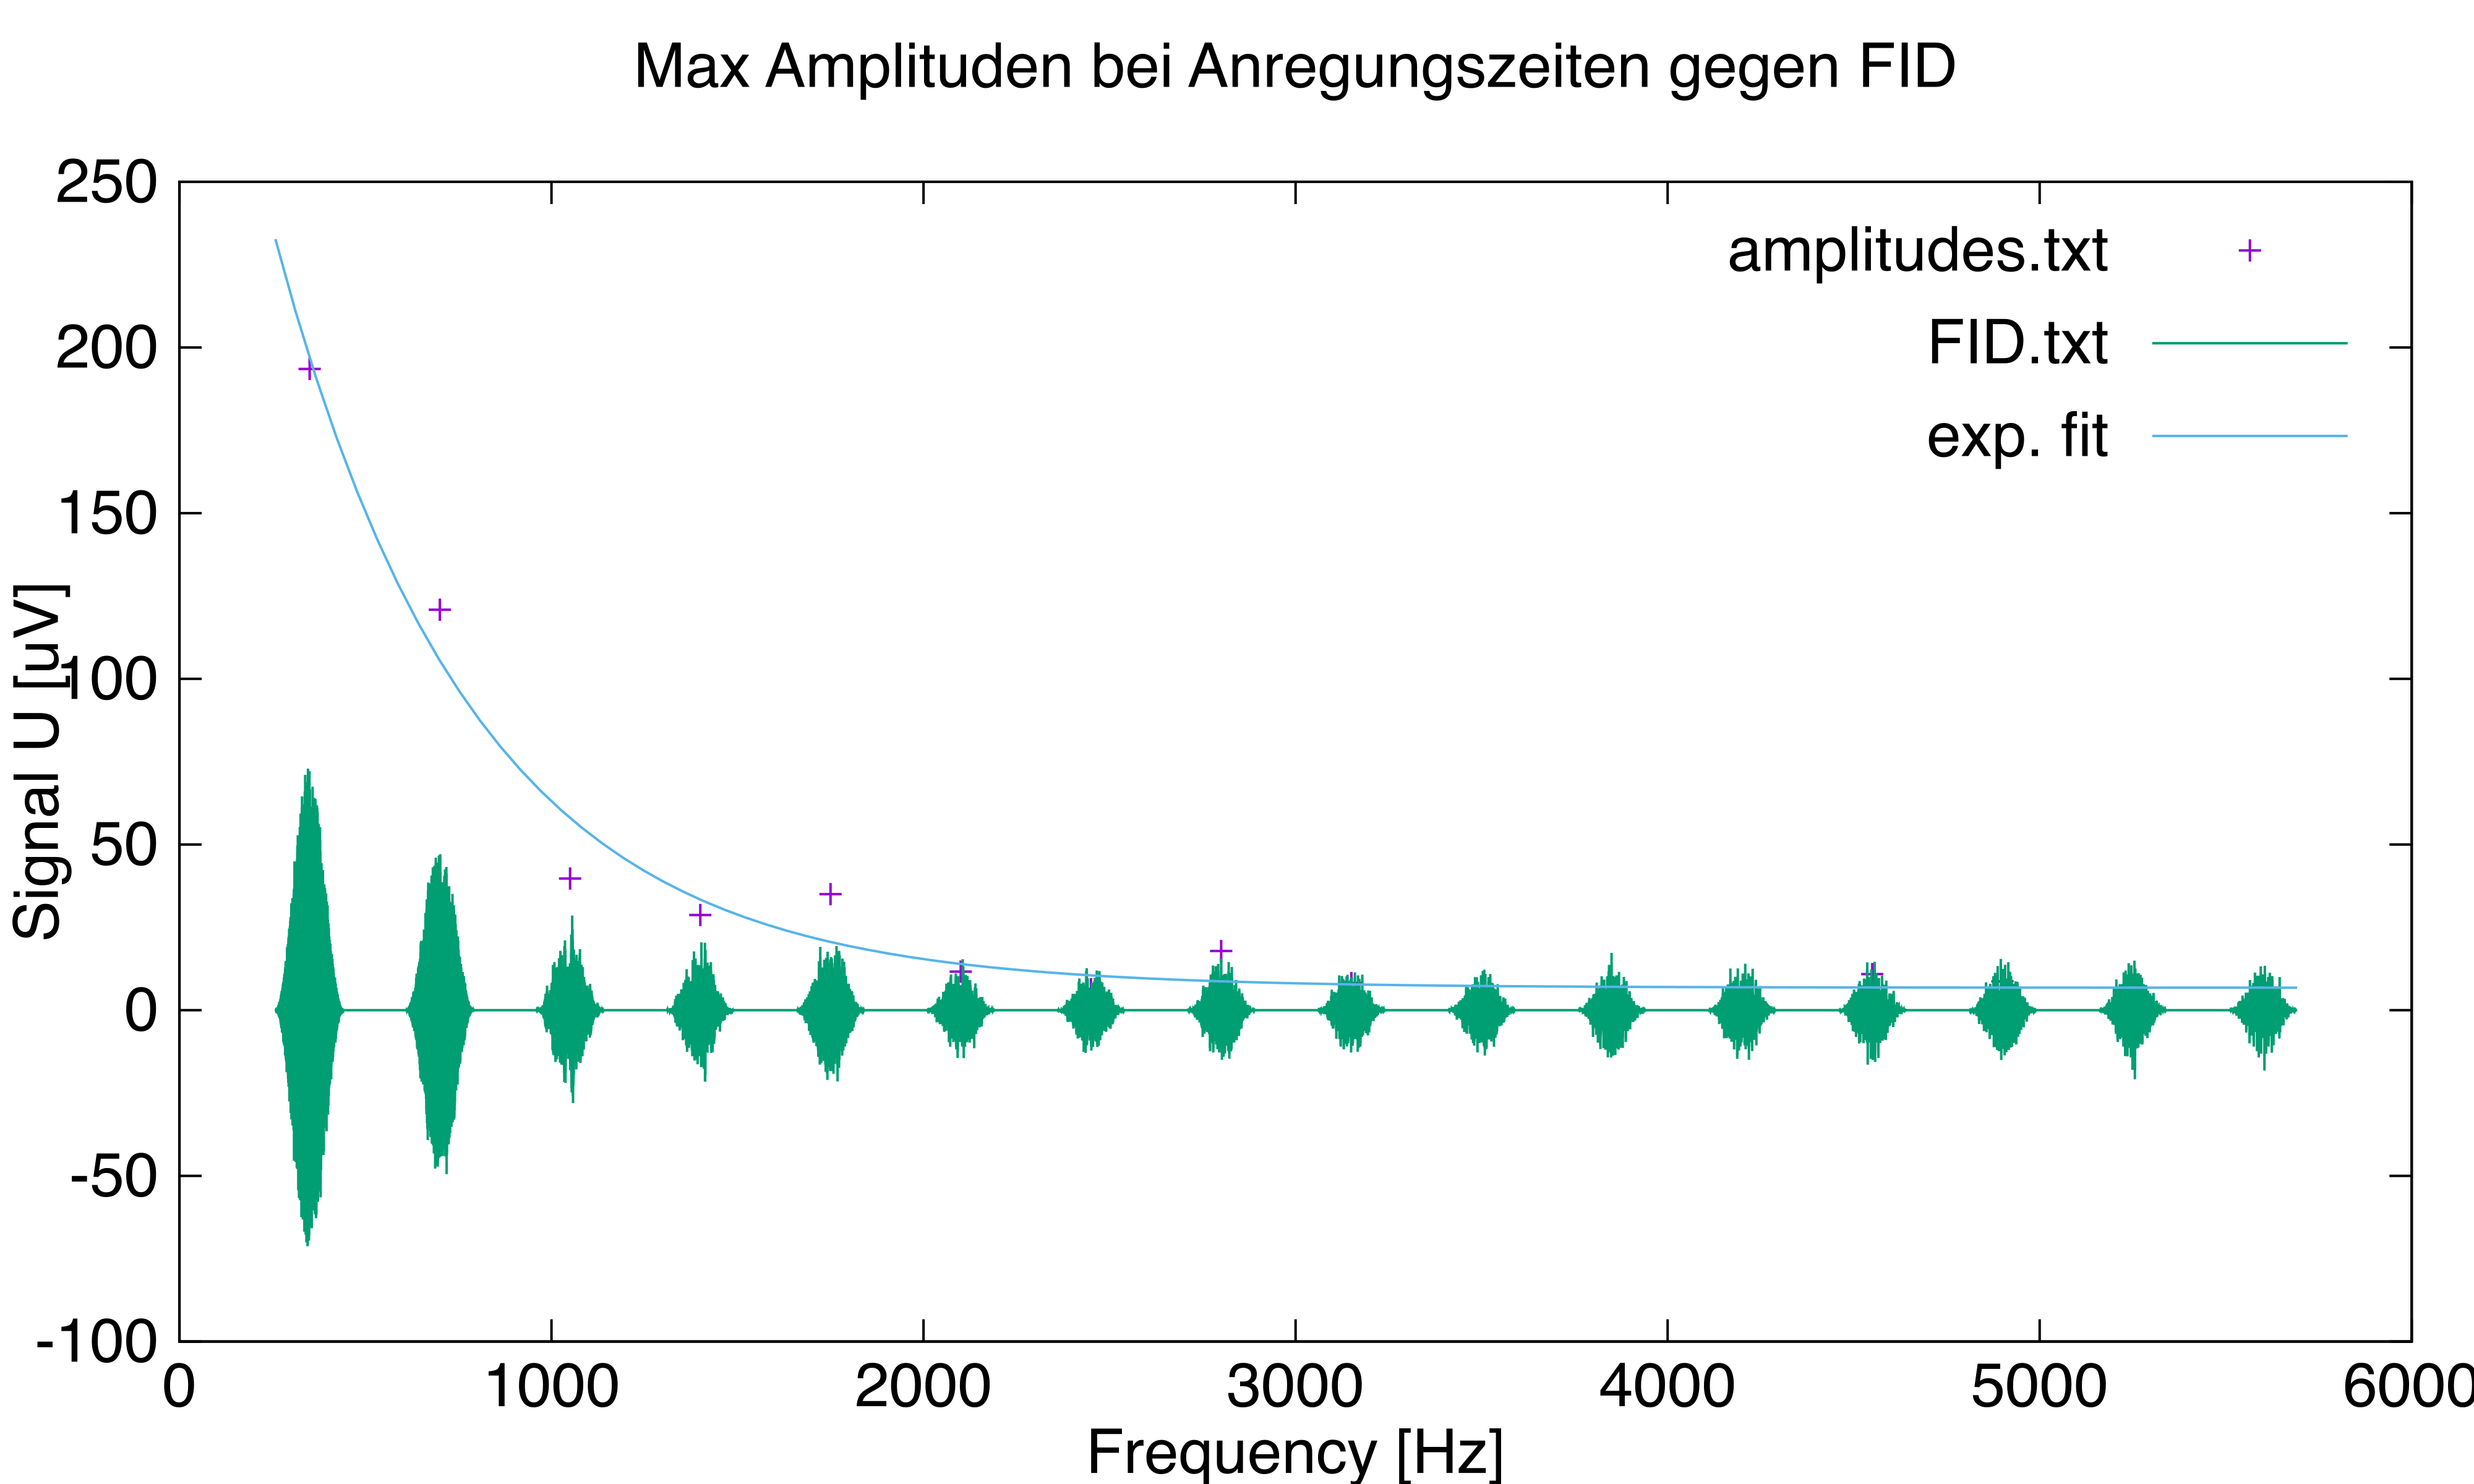
\includegraphics[width=6cm]{../Bilddateien/CPMG-90-270-constant-avg.png}
                \caption{mod. const.}
                \label{fig:CPMG-90-270-constant-avg}
            \end{subfigure}
            \
            \begin{subfigure}[b]{0.4\textwidth}
                \centering
                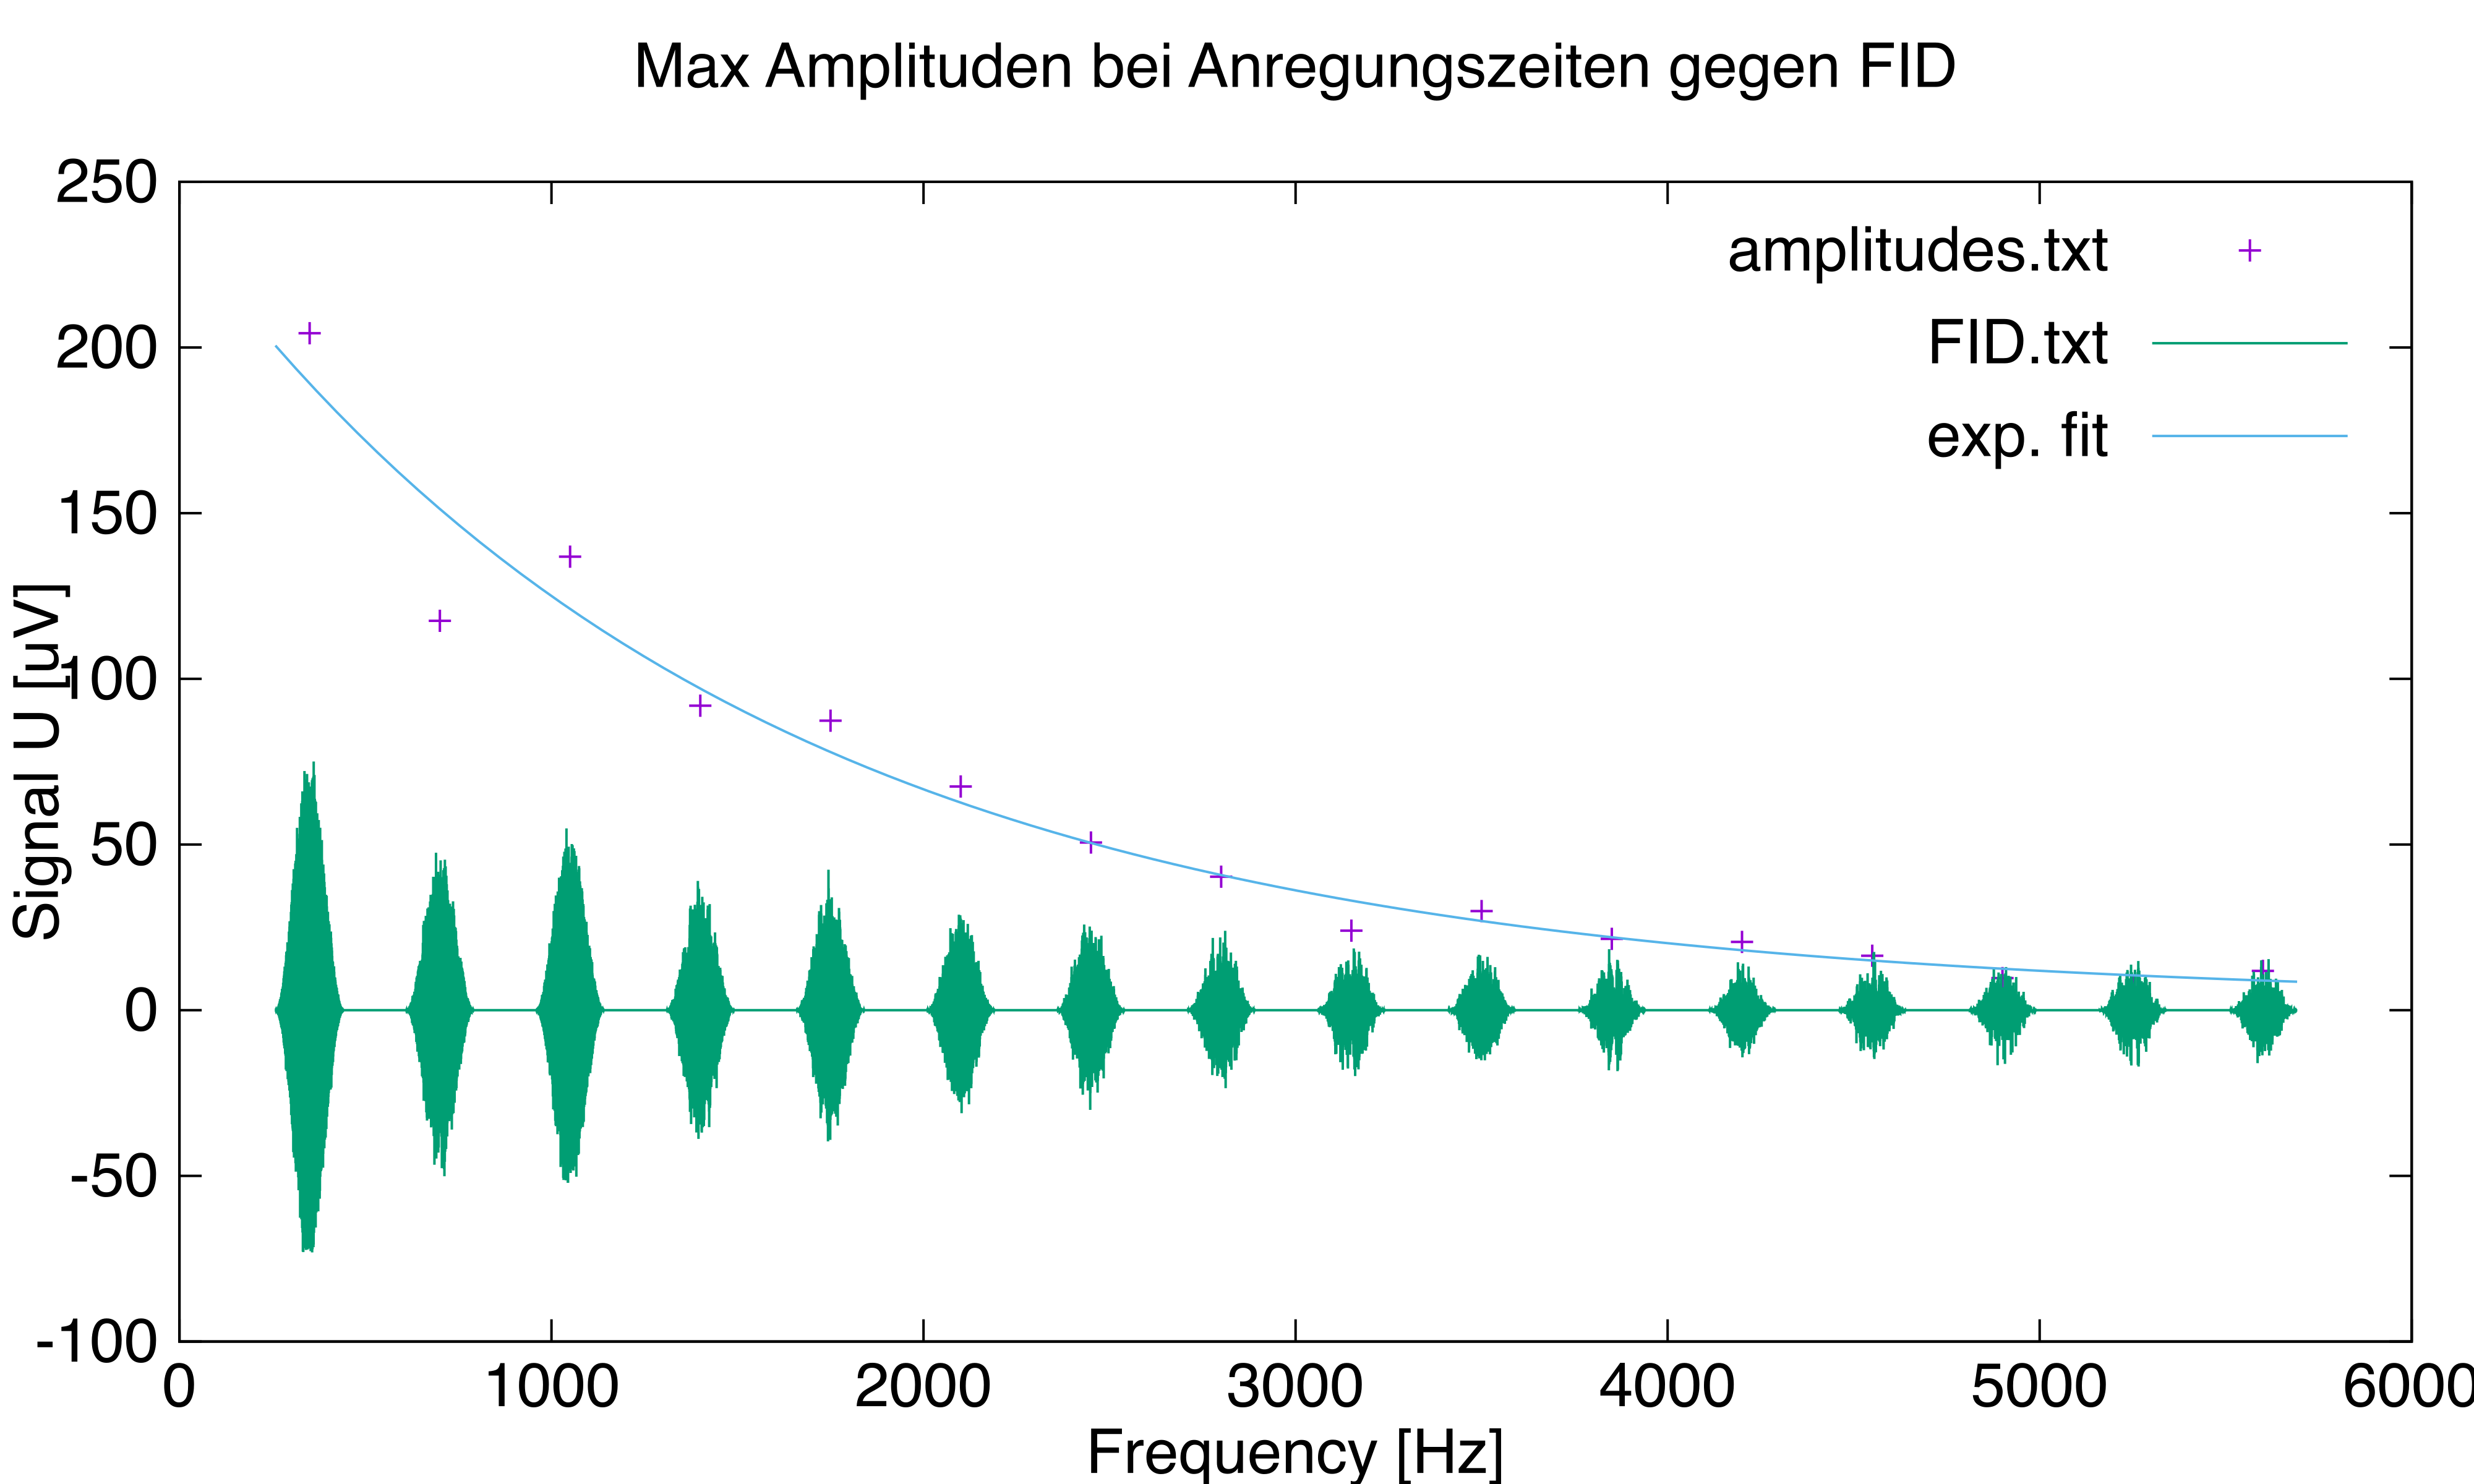
\includegraphics[width=6cm]{../Bilddateien/CPMG-90-270-alternating-avg.png}
                \caption{mod. alt.}
                \label{fig:CPMG-90-270-alternating-avg}
            \end{subfigure}
            \caption{FID und Amplitudensignale nichtnormiert und gemittelt für $\varphi_1 = 90$, $\varphi_2 = 270$.}
            \label{fig:CPMG-90-270-avg}
        \end{figure}
        
\end{document}